\documentclass[11pt]{article}

\usepackage[margin=1in]{geometry}
\usepackage{amsmath}
\usepackage{amssymb}
\usepackage{graphicx}
\usepackage{booktabs}
\usepackage{xcolor}
\usepackage[font=small,labelfont=bf,labelsep=period]{caption}
\usepackage[hidelinks]{hyperref}

% Symbols, one per object.
\newcommand{\kmax}{k_{\rm max}}
\newcommand{\hMpc}{\,h\,{\rm Mpc}^{-1}}
\newcommand{\aunit}{\,h^{-2}\,{\rm Mpc}^2}
\newcommand{\bstwo}{b_{s^2}}
\newcommand{\SNz}{{\rm SN}_0}
\newcommand{\SNt}{{\rm SN}_2}
\newcommand{\T}{^{\mathsf{T}}}
% The statistic of the error-bar test.  It has no name; its value is
% written \eta.
\newcommand{\chidof}{\sqrt{\langle\chi^2\rangle/n_{\rm dof}}}
% The clause of every caption with a k_max axis.
\newcommand{\kmaxclause}{$\kmax$ at $z = 0$; each bin is cut at
  $\kmax/D(\bar{z}_i)$.}

% =====================================================================
% Numbers: refresh after the converged-derivative recompute
% =====================================================================
% Every number the text quotes is defined in this section.  Part 1
% holds the forecast results: they come from the data.json files under
% plots/ and from the printed tables of section 9 of
% EXAMPLE_EVALUATE_FISHER_MODEL.ipynb, and they move whenever the
% Fisher derivatives change.  Part 2 holds the inputs (prior widths,
% drift sizes, survey numbers) and the properties of the templates,
% which the derivatives do not change.
%
% Every macro of Part 1 written as \refresh{...} comes from the
% final-tier run of EXAMPLE_EVALUATE_FISHER_MODEL.ipynb of 2026-11-10
% (section 9 and the summary_* data.json it wrote, on the scale cuts of
% the paper fiducial).  A
% later rerun refreshes them again: set \numbersfinalfalse to print them
% in red with a note under the title while they are out of date and the
% expensive derivatives are being recomputed, put in the
% new values, set \numbersfinaltrue, rebuild, and check the statements
% listed further down.  Part 2, Part 3 and the LSST Y1 values are not
% refreshed by that run.
%
% Layout suffixes: Com = Delta d_com = 62 Mpc, Two = Delta z = 0.02,
% Five = Delta z = 0.05, Twenty = Delta z = 0.2.  Low = k_max = 0.075,
% High = k_max = 0.2 (h/Mpc, at z = 0).
%
% Statements of the text that rest on Part 1; check each after a
% refresh:
%   - DESI C_ell^gg alone stays below LSST Y1 3x2pt in both FoMs at
%     every cut (Summary; the section "Forecast");
%   - the thin layouts carry most of the information: their
%     FoM(w0, wa) is the largest at every cut from k_max = 0.075 on
%     (the section "Forecast");
%   - "per bin, group width" lies above the model on every layout at
%     every cut from k_max = 0.075 on; "per bin, group width x sqrt(N)"
%     lies above it on Delta z = 0.2; "per bin, x sqrt(N) + group tilt"
%     stays at or below 1 (largest ratio 0.96); the costs fall from
%     k_max = 0.075 to 0.2; correlated residuals cost more than
%     independent per-bin terms on the three thinner layouts and nothing
%     on Delta z = 0.2 (the section "What the grouping is worth");
%   - "one constant value per wide sample" claims the largest FoM
%     ratios of the untied figure on every layout from k_max = 0.075
%     on; its sqrt(<chi^2>/n_dof) of (w0, wa) is larger at 0.2 than at
%     0.075 on every layout, and its smallest coverage sits on
%     Delta z = 0.02 (the section "What the grouping is worth");
%   - in the bottom row of the untied figure the four versions that
%     free b1 per bin sit exactly at 1, correlated residuals stay
%     within EtaCorrMin-EtaCorrMax, and the model within EtaW
%     (the section "What the grouping is worth");
%   - pairs beyond the list: the largest gains, their values with the
%     bias line fixed and with every nuisance parameter fixed, and the
%     agreement across the passing priors track the Pair* macros below
%     (the section "The cross pairs and their overlaps").
% ---------------------------------------------------------------------
% The refresh switch: \numbersfinalfalse prints every \refresh value in
% red and the note under the title; \numbersfinaltrue prints them plain.
\newif\ifnumbersfinal
\numbersfinaltrue
\newcommand{\refresh}[1]{\ifnumbersfinal#1\else\textcolor{red}{#1}\fi}
% A value the exploration tier does not have yet.
\newcommand{\pending}{[pending]}
% ---------------------------------------------------------------------
% Part 1: results.
%
% FoM(w0, wa) at k_max = 0.075 and 0.2 (summary_fom_kmax/data.json, fom)
\newcommand{\FoMwLowCom}{\refresh{0.564}}
\newcommand{\FoMwLowTwo}{\refresh{0.352}}
\newcommand{\FoMwLowFive}{\refresh{0.173}}
\newcommand{\FoMwLowTwenty}{\refresh{0.0447}}
\newcommand{\FoMwHighCom}{\refresh{6.70}}
\newcommand{\FoMwHighTwo}{\refresh{7.95}}
\newcommand{\FoMwHighFive}{\refresh{2.34}}
\newcommand{\FoMwHighTwenty}{\refresh{0.307}}
% FoM(Omega_m, 10^9 A_s) at k_max = 0.2 (summary_fom_kmax/data.json,
% fom_om_as)
\newcommand{\FoMoHighCom}{\refresh{50.3}}
\newcommand{\FoMoHighTwo}{\refresh{53.2}}
\newcommand{\FoMoHighFive}{\refresh{19.9}}
\newcommand{\FoMoHighTwenty}{\refresh{3.20}}
% LSST Y1 3x2pt alone, FoM(w0, wa) and FoM(Omega_m, 10^9 A_s): the
% lsst_y1 project's forecast (summary_fom_kmax/data.json, lsst_y1_*);
% not refreshed, since the DESI recompute leaves them unchanged
\newcommand{\LSSTw}{17.3}
\newcommand{\LSSTo}{215}
% The error-bar test under the known drifts plus a residual drawn from
% the prior (EXAMPLE_EVALUATE_FISHER_MODEL.ipynb, section 9): the
% largest sqrt(<chi^2>/n_dof) over layouts and cuts, overall and for
% (w0, wa), Omega_m and A_s, and the smallest coverage of the 1 sigma
% region
\newcommand{\EtaMax}{\refresh{1.030}}
\newcommand{\EtaW}{\refresh{1.019}}
\newcommand{\EtaOm}{\refresh{1.030}}
\newcommand{\EtaAs}{\refresh{1.004}}
\newcommand{\CoverMin}{\refresh{66.8\%}}
% Untying (summary_fom_untied/data.json, ratio_fom, from k_max = 0.075
% on).  A cost is 1/ratio.  CostNested*: the version nested ("per bin,
% on top of the model"): Low* its range on the two thin layouts at
% k_max = 0.075, High* its range on the three thinner layouts at 0.2.
% CostCorr*: the version correlated_residuals ("correlated residuals on
% top of the model"): Low* its range on the three thinner layouts at
% 0.075 (smallest on Delta d_com = 62 Mpc, largest on Delta z = 0.02);
% High* its range on the three thinner layouts at 0.2; it equals the
% model on Delta z = 0.2 (ratio 1).  WideMax: the largest cost of both
% versions on Delta z = 0.2 at any cut.  GainMax: the largest ratio of
% the version gauss ("per bin, group width"), Delta z = 0.02 at 0.1.
% FoMwSmallCut bounds the model's own FoM(w0, wa) at k_max = 0.05
% (largest 0.044, Delta z = 0.05).
\newcommand{\CostNestedLowMin}{\refresh{1.12}}
\newcommand{\CostNestedLowMax}{\refresh{1.17}}
\newcommand{\CostNestedHighMin}{\refresh{1.06}}
\newcommand{\CostNestedHighMax}{\refresh{1.13}}
\newcommand{\CostCorrLowMin}{\refresh{1.4}}
\newcommand{\CostCorrLowMax}{\refresh{1.8}}
\newcommand{\CostCorrHighMin}{\refresh{1.23}}
\newcommand{\CostCorrHighMax}{\refresh{1.29}}
\newcommand{\CostWideMax}{\refresh{1.13}}
\newcommand{\UntieGainMax}{\refresh{1.54}}
\newcommand{\FoMwSmallCut}{\refresh{0.05}}
% The version constant_per_sample ("one constant value per wide
% sample") of summary_fom_untied/data.json, from k_max = 0.075 on.
% ConstGainLow*: its ratio_fom over the layouts at 0.075 (smallest on
% Delta d_com = 62 Mpc, largest on Delta z = 0.2); ConstGainHigh*: the
% same at 0.2 (smallest on Delta d_com = 62 Mpc, largest on
% Delta z = 0.2); ConstGainTwenty*: its ratio_fom on Delta z = 0.2 over
% the cuts; ConstGainOm*: its ratio_fom_om_as over layouts and cuts.
% ConstEta*: its eta of (w0, wa) over the layouts at 0.075 and at 0.2,
% and its eta of Omega_m and of A_s at 0.2 (over all cuts from 0.075 on
% the Omega_m value peaks at 3.8, on Delta d_com = 62 Mpc at 0.1; the
% text quotes 0.2).
% ConstCover*: the smallest coverage per layout over (w0, wa), Omega_m
% and A_s: its range over the layouts, and the smallest anywhere
% (ConstCoverWorst), (w0, wa) on Delta z = 0.02 at 0.2.  ConstEvo*: the
% shift of
% (w0, wa) under the bias's own evolution inside each sample alone,
% over the layouts at 0.075 and at 0.2 (evolution_shift) [sigma].
% EtaCorr*: the range of the version correlated_residuals in eta of
% (w0, wa) over layouts and cuts from 0.075 on.
\newcommand{\ConstGainLowMin}{\refresh{2.4}}
\newcommand{\ConstGainLowMax}{\refresh{7.5}}
\newcommand{\ConstGainHighMin}{\refresh{2.1}}
\newcommand{\ConstGainHighMax}{\refresh{3.2}}
\newcommand{\ConstGainTwentyMin}{\refresh{3.2}}
\newcommand{\ConstGainTwentyMax}{\refresh{7.5}}
\newcommand{\ConstGainOmMin}{\refresh{1.5}}
\newcommand{\ConstGainOmMax}{\refresh{5.1}}
\newcommand{\ConstEtaLowMin}{\refresh{2.2}}
\newcommand{\ConstEtaLowMax}{\refresh{3.4}}
\newcommand{\ConstEtaHighMin}{\refresh{2.9}}
\newcommand{\ConstEtaHighMax}{\refresh{6.4}}
\newcommand{\ConstEtaOm}{\refresh{3.0}}
\newcommand{\ConstEtaAs}{\refresh{4.7}}
\newcommand{\ConstCoverMin}{\refresh{5\%}}
\newcommand{\ConstCoverMax}{\refresh{11\%}}
\newcommand{\ConstCoverWorst}{\refresh{5.0\%}}
\newcommand{\ConstEvoLowMin}{\refresh{3.8}}
\newcommand{\ConstEvoLowMax}{\refresh{6.0}}
\newcommand{\ConstEvoHighMin}{\refresh{4.7}}
\newcommand{\ConstEvoHighMax}{\refresh{17}}
\newcommand{\EtaCorrMin}{\refresh{0.99}}
\newcommand{\EtaCorrMax}{\refresh{1.01}}
% Pairs beyond the current list (the gap and sigma_v axes of
% notes/cross_correlations).  PairGain*: the largest FoM(w0, wa) ratio
% to the current data vector of each thinner layout, sigma_v fitted,
% over the two cuts the figure draws (plots/summary_pair_axes/
% data.json: 62 Mpc and Delta z = 0.05 at k_max = 0.075,
% Delta z = 0.02 at 0.2); PairGainOm: the largest
% FoM(Omega_m, 10^9 A_s) ratio (Delta z = 0.05 at 0.075);
% PairGainTwentyMax bounds Delta z = 0.2 at every cut.  PairLine*: the
% same ratios with each group's bias line (the level and slope of the
% amplitudes beta) held fixed; PairNuisMax: the largest ratio anywhere
% with every nuisance parameter held fixed (62 Mpc at 0.075; both from
% plots/summary_pair_attribution/data.json).  PairPriorSpread: the
% largest difference of the ratio across the three passing linear-bias
% priors (notes/cross_correlations, plots/pair_axes_priors/data.json).
\newcommand{\PairGainCom}{\refresh{1.55}}
\newcommand{\PairGainTwo}{\refresh{1.44}}
\newcommand{\PairGainFive}{\refresh{1.59}}
\newcommand{\PairGainOm}{\refresh{1.44}}
\newcommand{\PairGainTwentyMax}{\refresh{$2\%$}}
\newcommand{\PairLineCom}{\refresh{1.29}}
\newcommand{\PairLineFive}{\refresh{1.08}}
\newcommand{\PairNuisMax}{\refresh{$8\%$}}
\newcommand{\PairPriorSpread}{\refresh{$3\%$}}
% ---------------------------------------------------------------------
% Part 2: inputs and template properties (not moved by the recompute).
%
% The linear-bias residual: width, correlation length, and the rms
% difference of two neighbors at Delta z = 0.02,
% sigma_g [2(1 - exp(-0.02/L))]^(1/2)
\newcommand{\sigG}{3\%}
\newcommand{\Lcorr}{0.05}
\newcommand{\NeighborRms}{2.4\%}
% Widths of the Gaussian priors, all centered on zero
\newcommand{\wDtwo}{2}
\newcommand{\wDs}{1}
\newcommand{\wSNz}{2}
\newcommand{\wSNt}{5}
% Counterterms: a correction ctFrac at the cut, a width ctFrac/k_max^2,
% which is ctDESI h^-2 Mpc^2 at 0.2 h/Mpc
\newcommand{\ctFrac}{0.5}
\newcommand{\ctDESI}{12.5}
% What the offset widths hedge (notes/higher_order_bias): the spread of
% co-evolution against excursion-set tidal biases, and the largest
% share of the loops in the galaxy power at the shipped mask
\newcommand{\CoevSpread}{30\%}
\newcommand{\LoopShare}{15\%}
% The known drifts (notes/correlated_bias_prior_v2): a conserved
% population's departure from B_g/D per Delta z = 0.05; the BGS
% r < 19.5 flux-limit drift across the group and the rms its best line
% leaves; the redshift span of the 4000 A break crossing a filter edge;
% the finest redshift scale on which the bias is measured
\newcommand{\ConsDrift}{1\%}
\newcommand{\BGSspan}{22\%}
\newcommand{\BGScurv}{2.4\%}
\newcommand{\FilterDzMin}{0.03}
\newcommand{\FilterDzMax}{0.05}
\newcommand{\MeasuredDz}{0.1}
% The SN2 template (notes/higher_order_bias): the median normalized
% adjacent cross term over the adjacent pairs of one sample on
% Delta d_com = 62 Mpc, the same for SN0, and the number of pairs
\newcommand{\SNtAdj}{-0.50}
\newcommand{\SNzAdj}{+0.05}
\newcommand{\NadjPairs}{73}
% SN2 units, (f_sat, sigma_sat [h^-1 Mpc]) of LRG and ELG
\newcommand{\fsat}{0.1}
\newcommand{\ssatLRG}{7.8}
\newcommand{\ssatELG}{2.9}
% The survey: covariance and forecast areas [deg^2]; bins per layout;
% band powers; the radial resolution of a 62 Mpc bin [h/Mpc]; the
% shipped mask [h/Mpc]
\newcommand{\AreaCov}{14{,}000}
\newcommand{\AreaSurvey}{12{,}300}
\newcommand{\NbinsCom}{76}
\newcommand{\NbinsTwo}{90}
\newcommand{\NbinsFive}{36}
\newcommand{\NbinsTwenty}{10}
\newcommand{\Nbands}{53}
\newcommand{\KparCom}{0.075}
% The measured cross pairs on Delta d_com = 62 Mpc: in all, in the DESI
% pair list, and the added LRG3 x ELG1 pairs (notes/cross_correlations)
\newcommand{\NcrossCom}{107}
\newcommand{\NcrossDESI}{97}
\newcommand{\NcrossExtra}{ten}
% The correlation length of the residuals added in the untied version
% "correlated residuals on top of the model" (b1's L)
\newcommand{\LcorrHO}{0.05}
% The toy example of Section 6: N bins of the group width of Delta_2
% (wDtwo); the width of their average, wDtwo/sqrt(ToyN); and the factor
% by which it is tighter than the group width
\newcommand{\ToyN}{9}
\newcommand{\ToyAvg}{2/3}
\newcommand{\ToyFactor}{three}
\newcommand{\kMask}{0.176}
% The pair rule and the overlap studies (section 11, items 6 and 7, of
% EXAMPLE_EVALUATE_FISHER_MODEL.ipynb; plots/summary_pair_threshold/
% data.json, now the paper model's own scan, and
% notes/fog_parameter_degeneracy_study/plots/
% fog_pair_overlap/data.json).  The overlaps depend only on the n(z)
% and sigma_v, never on the derivatives; the FoM ratios are refreshed
% with them.  PairCoarse*: the Delta z = 0.2
% FoM ratios at O_min = 1e-2, at k_max = 0.075 and 0.2 (the two cuts the
% figure draws).
\newcommand{\OvThreshold}{10^{-6}}
\newcommand{\OvGapTop}{0.028}
\newcommand{\OvBoundary}{3.4\times10^{-7}}
\newcommand{\OvListGapTop}{3.4\times10^{-3}}
\newcommand{\PairDropCost}{\refresh{$0.2\%$}}
\newcommand{\PairCoarseMin}{\refresh{0.89}}
\newcommand{\PairCoarseMax}{\refresh{0.95}}
\newcommand{\PairCoarseOmMin}{\refresh{0.77}}
\newcommand{\PairCoarseOmMax}{\refresh{0.87}}
% The sigma_v axis of the pairs-beyond-the-list study selects its
% lists with the same overlap criterion, every dispersion set to one
% common value s: the s [km/s] at which the first pair beyond the
% current data vector passes the threshold, per layout (the pair
% counts of notes/cross_correlations, plots/pair_axes_sigv/data.json;
% Delta z = 0.2 never adds a pair).
\newcommand{\SvJoinTwo}{450}
\newcommand{\SvJoinCom}{750}
\newcommand{\SvJoinFive}{1200}
% The Fingers-of-God dispersions (likelihood/params_desi*_bias_
% pessimistic.yaml; the fiducial section holds the per-group table):
% the base widths [km/s] (five times the median per-bin uncertainty of
% the dispersion measurements), the widening factor of the priors, and
% the truncated mean of the BGS0 prior [km/s].
\newcommand{\SigBase}{$145$, $105$, $70$, $50$, $50$, $40$, $30$}
\newcommand{\SigVfactor}{six}
\newcommand{\BGSzeroMean}{847}
% ---------------------------------------------------------------------
% Part 3: the Fisher machinery and its convergence (notes/fisher_machinery,
% sections "The base, and every model as a matrix on it", "Derivative
% accuracy", "A scale cut is a set of rows").  These values come from the convergence study
% (tests/studies/run_fisher_derivatives.py) and the builders; the ones
% marked \refresh are the paper model's FoM ratios of
% plots/fom_convergence/data.json (the study's derivatives rescored on
% the paper-fiducial cuts), which move with the cuts; the rest the
% final run of EXAMPLE_EVALUATE_FISHER_MODEL.ipynb does not refresh.
%
% The stencil step (relative); the pseudo-inverse: the eigenvalue
% threshold relative to the largest, and the largest component a
% dropped direction may have on (w0, wa), Omega_m or A_s
\newcommand{\StepH}{0.02}
\newcommand{\PinvTol}{10^{-12}}
\newcommand{\PinvTouch}{10^{-6}}
% Batching: batches per layout, evaluations per per-bin family
\newcommand{\Nbatch}{four}
\newcommand{\NevalFamily}{16}
% The MCMC chi^2 criterion; what MCMC-grade settings do to
% FoM(w0, wa) on Delta z = 0.05 at k_max = 0.075 and 0.2
% (fom_convergence/data.json, points.mcmc)
\newcommand{\MCMCdchi}{0.2}
\newcommand{\ConvMCMCLow}{\refresh{56\%}}
\newcommand{\ConvMCMCHigh}{\refresh{13\%}}
% The grids: the converged grid, the study's starting grid, the final
% grid, the MCMC grid of Delta z = 0.05 and the ratio of the last two;
% the distances per unit of grid factor
\newcommand{\GridConv}{512}
\newcommand{\GridStart}{128}
\newcommand{\GridFinal}{256}
\newcommand{\GridMCMC}{32}
\newcommand{\GridRatio}{eight}
\newcommand{\GridUnit}{511}
% The final settings: CosmoLike accuracyboost and integration_accuracy;
% CAMB AccuracyBoost, k_per_logint, maximum wavenumber [1/Mpc]; the
% halofit bisection tolerance, stock and patched
\newcommand{\FinAccBoost}{3}
\newcommand{\FinIntAcc}{1}
\newcommand{\FinCambBoost}{2.0}
\newcommand{\FinKlog}{30}
\newcommand{\FinKmax}{60}
\newcommand{\HalofitStock}{10^{-3}}
\newcommand{\HalofitPatch}{10^{-7}}
% The study's starting configuration (g = GridStart with every other
% control raised; the grid scan holds these other controls): CosmoLike
% accuracyboost and integration_accuracy, low-rank rank and multipole
% cap, CAMB AccuracyBoost, k_per_logint, maximum wavenumber [1/Mpc].
% It is not the final setting (g = GridFinal) and not the converged one
% (g = GridConv).
\newcommand{\StartAccBoost}{4}
\newcommand{\StartIntAcc}{2}
\newcommand{\StartRank}{8}
\newcommand{\StartCap}{2000}
\newcommand{\StartCambBoost}{2}
\newcommand{\StartKlog}{30}
\newcommand{\StartKmax}{80}
% The final settings against the converged value on Delta z = 0.05:
% FoM(w0, wa) and FoM(Omega_m, 10^9 A_s) at k_max = 0.075 and 0.2, the
% largest change of a marginalized error, the largest change of a shift
% [sigma]; the step independence from h/2 to 3h on Delta z = 0.05 and
% on Delta d_com = 62 Mpc
\newcommand{\ConvFoMwLow}{\refresh{$+2.1\%$}}
\newcommand{\ConvFoMwHigh}{\refresh{$-0.5\%$}}
\newcommand{\ConvFoMoLow}{\refresh{$+1.8\%$}}
\newcommand{\ConvFoMoHigh}{\refresh{$-0.4\%$}}
\newcommand{\ConvSigma}{1.6\%}
\newcommand{\ConvShift}{0.007}
\newcommand{\ConvStep}{\refresh{1.6\%}}
\newcommand{\ConvStepCom}{\refresh{0.5\%}}
% DerivKit: its least number of evaluations per column, and its
% agreement with the stencils at the final settings
\newcommand{\DkitPoints}{seven}
\newcommand{\DkitAgree}{2.1\%}
% The setter route against the study's untied-parameter route: b1, and
% the stencil columns (b2, bs2 and alpha_0 agree exactly)
\newcommand{\RouteBone}{5\times10^{-11}}
\newcommand{\RouteStencil}{5\times10^{-14}}
% The cost: evaluations of the data vector per layout, seconds per
% evaluation at the final settings, hours per thin layout
\newcommand{\Neval}{154}
\newcommand{\TevalMin}{20}
\newcommand{\TevalMax}{40}
\newcommand{\HoursMin}{one}
\newcommand{\HoursMax}{two}
% =====================================================================

\emergencystretch=2em
% One-column figures keep their natural width (made for one column of a
% two-column paper) and carry their caption at their side; \sidegap is
% the space between figure and caption.
\newlength{\sidegap}
\setlength{\sidegap}{0.22in}
% let a figure share a page with text; no figure-only pages
\renewcommand{\topfraction}{0.9}
\renewcommand{\bottomfraction}{0.8}
\renewcommand{\textfraction}{0.07}
\renewcommand{\floatpagefraction}{0.85}
\setcounter{topnumber}{3}
\setcounter{totalnumber}{4}

\begin{document}

\begin{center}
  {\LARGE The galaxy-bias model of the lssty1xdesi paper\par}
  \vspace{0.6em}
  {\large One model and one prior for DESI $C_\ell^{gg}$ in thin
    redshift bins\par}
  \vspace{0.6em}
  {\large November 2026\par}
  \ifnumbersfinal\else
    \vspace{0.6em}
    {\color{red}Numbers in red are being refreshed with the final-tier
      Fisher derivatives.\par}
  \fi
\end{center}
\vspace{1em}

\section{Summary}
\label{sec:summary}

\paragraph{The question.}
What does DESI galaxy clustering, measured as angular power spectra
$C_\ell^{gg}$ in thin redshift bins, constrain on its own, with a bias
model a referee accepts?  Thin bins resolve the growth of structure
along the line of sight only if the bias of neighboring bins is not
free bin by bin; tying the bins too tightly instead turns assumptions
about the bias into cosmology.

\paragraph{The model.}
The fiducial model's galaxy power spectrum is one-loop, with seven
bias quantities per
bin: the linear, quadratic and tidal biases, the counterterms
$\alpha_0$ and $\alpha_2$, and the stochastic terms $\SNz$ and $\SNt$.
Each of them is its group's value, which follows calibrations where
they exist, plus, depending on the quantity, a free tilt in redshift
across the group and a residual of the bin with a Gaussian prior
correlated in redshift (Section~\ref{sec:model}).  The line-of-sight
counterterm is fixed, $\alpha_2 = 0$ in every bin: the sampled
Fingers-of-God dispersions, whose priors are widened \SigVfactor{}-fold,
carry that freedom instead.  One principle sets
the priors: slicing a wide DESI sample into thin bins adds measurements
but no knowledge of the bias, so the group value and the tilt carry
exactly the freedom of the wide sample, and the residual is what the
slicing may add within it (Section~\ref{sec:prior}).

\paragraph{The result.}
On the two thin layouts, ${\rm FoM}(w_0, w_a)$ of DESI $C_\ell^{gg}$
alone grows from \FoMwLowCom{} and \FoMwLowTwo{} at
$\kmax = 0.075\hMpc$ to \FoMwHighCom{} and \FoMwHighTwo{} at $0.2\hMpc$,
below the \LSSTw{} of LSST Y1 3x2pt alone; ${\rm FoM}(\Omega_m, 10^9
A_s)$ stays below LSST Y1 as well (Section~\ref{sec:forecast}).  Over
random bias histories, the known drifts plus scatter drawn from the
prior, the quoted error bars are honest at every cut and on every
layout (Section~\ref{sec:forecast}).

\paragraph{Pairs beyond the list.}
Cross spectra of bins further apart than the pair list measures
would raise ${\rm FoM}(w_0, w_a)$ by up to a factor of \PairGainCom{}
on the thin layouts (Section~\ref{sec:pairs}).  The gain rests on the
freedom the prior grants: each group's free bias level and slope
mimic the growth history in the auto spectra, the added cross
spectra separate the two, and with that level and slope held fixed
most of the gain goes.  The analysis keeps the current data vector;
the longer lists are a comparison against it.  Open is a finite
prior on the levels and slopes.

\paragraph{What the grouping is worth.}
A per-bin prior that looks looser than the model gains information by
accident, from the slicing alone, up to a factor of \UntieGainMax{} in
${\rm FoM}(w_0, w_a)$.  Untied bins that keep the freedom of the wide
samples cost a factor of \CostNestedLowMin{} to \CostNestedLowMax{} in
${\rm FoM}(w_0, w_a)$ on the thin layouts at $\kmax = 0.075\hMpc$ with
independent per-bin terms, and up to \CostCorrLowMax{} with residuals
correlated in redshift (Section~\ref{sec:grouping}).  One constant
value of every bias quantity per wide sample claims up to
\ConstGainLowMax{} times the model's ${\rm FoM}(w_0, w_a)$, with error
bars up to \ConstEtaHighMax{} times too small.

\section{Fiducial model and parameter values}
\label{sec:fiducial}

Every number of this note was computed at the fiducial below, the
evaluate point of the paper configurations
\texttt{EXAMPLE\_EVALUATE1}--\texttt{4.yaml}, frozen here so the note
does not depend on files that may change.

\paragraph{Cosmology.}
Flat $w_0 w_a$CDM: $10^9 A_s = 2.1$, $n_s = 0.96605$,
$H_0 = 67.32$~km/s/Mpc, $\Omega_b = 0.04$, $\Omega_m = 0.3$ (neutrinos
included), $w_0 = -1$ and $w_0 + w_a = -1$, so $w_a = 0$; derived
$\sigma_8 = 0.8278$.  The Fisher matrices vary $10^9 A_s$, $n_s$,
$H_0$, $\Omega_b$, $\Omega_m$, $w_0$ and $w_a$ with flat priors; the
neutrino mass sum stays at $0.06$~eV and the optical depth at
$\tau = 0.0697$.

\paragraph{Layouts.}
Every layout carries \Nbands{} band powers per spectrum over
$15 \le \ell \le 544$ (Section~\ref{sec:data}).

\begin{center}
  \begin{tabular}{lccc}
    \toprule
    layout & lens bins & cross pairs & entries \\
    \midrule
    $\Delta d_{\rm com} = 62$~Mpc & 76 & 107 & 10{,}494 \\
    $\Delta z = 0.02$ & 90 & 133 & 12{,}614 \\
    $\Delta z = 0.05$ & 36 & 52 & 5{,}459 \\
    $\Delta z = 0.2$ & 10 & 13 & 2{,}014 \\
    \bottomrule
  \end{tabular}
\end{center}

\paragraph{Bias.}
The group amplitudes are $B_g = 1.34$ (BGS), $1.7$ (LRG1, LRG2, LRG3)
and $0.84$ (ELG1, ELG2), each flat in $[0.8, 4]$; at the fiducial every
tilt and residual is zero, so bin $i$ has
$b_{1,i} = B_g/D(\bar{z}_i)$, with the growth factor $D$ read off the
linear power spectrum at $k = 0.005~{\rm Mpc}^{-1}$.  The quadratic and
tidal biases sit on their calibrations, Eq.~\eqref{eq:calibrations}
with zero offsets, and every counterterm and stochastic amplitude is
zero: $\alpha_0 = \alpha_2 = \SNz = \SNt = 0$.  The linear-bias
residual prior has $\sigma_g = \sigG$ in every group and $L = \Lcorr$
(Section~\ref{sec:prior}).

\paragraph{Fingers-of-God dispersions.}
Seven dispersion groups: the six bias groups, with BGS split at
$\bar{z} = 0.255$ into BGS0 and BGS1.  Each has a Gaussian prior
centered on its fiducial, with a width \SigVfactor{} times its base
width (Section~\ref{sec:model}):

\begin{center}
  \begin{tabular}{lccccccc}
    \toprule
    {[km/s]} & BGS0 & BGS1 & LRG1 & LRG2 & LRG3 & ELG1 & ELG2 \\
    \midrule
    fiducial (prior center) & 371 & 358 & 357 & 348 & 343 & 304 & 289 \\
    base width & 145 & 105 & 70 & 50 & 50 & 40 & 30 \\
    prior width & 870 & 630 & 420 & 300 & 300 & 240 & 180 \\
    \bottomrule
  \end{tabular}
\end{center}

The sampled priors are truncated at zero.  The truncation matters most
for BGS0, whose prior width exceeds its center: the truncated prior's
mean is about $\BGSzeroMean$~km/s, not the $371$~km/s center.  The
Fisher forecast treats every $\sigma_v$ prior as an untruncated
Gaussian of the stated width.

\paragraph{Scale cuts.}
The UV-fraction cuts of every figure (Section~\ref{sec:data}) are
computed on this fiducial, from the paper configurations, at the
final derivative tier of Section~\ref{sec:method} -- the settings of
the derivative base -- and cached in
\begin{center}
  \texttt{chains/model\_scale\_cuts\_final.npz}.
\end{center}

\paragraph{Covariance.}
Gaussian, computed at this same fiducial with massless neutrinos (the
only difference from the data vector), at the fiducial dispersions,
for \AreaCov{} square degrees; every Fisher matrix rescales its
inverse to \AreaSurvey{} (Section~\ref{sec:method}).

\paragraph{Derivative tier.}
Five-point stencils at relative step $h = \StepH$, at the final
settings of the convergence study (Section~\ref{sec:method}): grid
factor $g = \GridFinal$, CosmoLike \texttt{accuracyboost}
\FinAccBoost{} and \texttt{integration\_accuracy} \FinIntAcc{}, CAMB
\texttt{AccuracyBoost} \FinCambBoost{}, \texttt{k\_per\_logint}
\FinKlog{}, maximum wavenumber \FinKmax{}~Mpc$^{-1}$ and the halofit
tolerance patch.  The base is cached in
\begin{center}
  \texttt{chains/model\_derivatives\_<layout>\_final.npz}
  \\ and \texttt{chains/model\_templates\_<layout>\_final.npz},
\end{center}
one pair per layout above.

\paragraph{The LSST Y1 3x2pt reference.}
The reference values \LSSTw{} and \LSSTo{} are the lsst\_y1 project's
real-space Fisher forecast of the SRD 3x2pt analysis.  Its fiducial
differs from this note's: $w_0 = -0.9$, and nonzero photo-z-shift and
shear-calibration centers, under Gaussian priors of widths $0.002$ and
$0.005$.

\section{Data and scale cut}
\label{sec:data}

The data are the DESI angular galaxy power spectra $C_\ell^{gg}$ in
\Nbands{} bands of width $\Delta\ell = 10$ over $15 \le \ell \le 544$,
with $\ell$ the multipole: the auto spectrum of every redshift bin and
the cross spectra of neighboring and overlapping bins.  On
$\Delta d_{\rm com} = 62$~Mpc these are \NcrossCom{} pairs: the
\NcrossDESI{} of the DESI forecast's pair list and \NcrossExtra{} LRG3$\times$ELG1
pairs at the same redshift, whose Fingers-of-God-blurred kernels
overlap (Section~\ref{sec:pairs}).  The galaxies
form six tracer groups $g$, each a wide sample selected as a whole: BGS
(the Bright Galaxy Survey), \mbox{LRG1--3} (luminous red galaxies) and
\mbox{ELG1--2} (emission-line galaxies).  Four layouts slice them:
$\Delta d_{\rm com} = 62$~Mpc, \NbinsCom{} bins of equal comoving width,
and $\Delta z = 0.02$, $0.05$ and $0.2$, with \NbinsTwo{}, \NbinsFive{}
and \NbinsTwenty{} bins of fixed redshift width.  The first two are the
thin layouts: a bin of comoving width $\Delta\chi$ resolves
line-of-sight wavenumbers up to $k_\parallel \simeq \pi/\Delta\chi$,
about \KparCom{}$\hMpc$ for the 62~Mpc bins, so thin bins keep much of
the three-dimensional information~\cite{Asorey2012}.  Bin $i$ has mean
redshift $\bar{z}_i$, and $D(z)$ is the linear growth factor,
$D(0) = 1$.

\paragraph{Parameters and figures of merit.}
Seven cosmological parameters vary with flat priors: $10^9 A_s$, with
$A_s$ the amplitude of the primordial curvature power spectrum; the
spectral index $n_s$; the Hubble constant $H_0$; the baryon and matter
densities today, $\Omega_b$ and $\Omega_m$, in units of the critical
density; and $w_0$ and $w_a$ of the dark-energy equation of state
$w_0 + w_a(1 - a)$, with $a$ the scale factor.  Seven Fingers-of-God
velocity dispersions $\sigma_v$, which smooth the bins' redshift
distributions, vary under the Gaussian priors of
Section~\ref{sec:fiducial} (widened to carry the line-of-sight
counterterm's freedom, Section~\ref{sec:model}).  With $\sigma$ a
parameter's
marginalized one-sigma error, ${\rm FoM}(w_0, w_a) = [\det {\rm
Cov}(w_0, w_a)]^{-1/2}$ is the inverse area of the marginalized
$(w_0, w_a)$ ellipse, and ${\rm FoM}(\Omega_m, 10^9 A_s)$ is defined the
same way.  The reference is LSST Y1 3x2pt alone~\cite{DESCSRD2018}: the
lsst\_y1 project's real-space Fisher forecast of the SRD analysis,
whose fiducial differs from this note's (Section~\ref{sec:fiducial}).

\paragraph{The scale cut.}
Matter is less nonlinear at higher redshift, so bin $i$ is cut at
$\kmax/D(\bar{z}_i)$, and every $\kmax$ here is the $z = 0$ value.  The
cut is the non-Limber UV-fraction criterion of Saraivanov et
al.~\cite{Saraivanov2026}, after DeRose and Chen~\cite{DeRoseChen2025}:
each band power splits into $C_\ell^{\rm IR}$, from the power spectrum
below the bin's cut wavenumber, and $C_\ell^{\rm UV}$, from the power
above it, and a band is kept while
\begin{equation}
  \frac{|C_\ell^{\rm UV}|}{|C_\ell^{\rm UV}| + |C_\ell^{\rm IR}|}
  \;<\; 0.05
  \label{eq:uvfraction}
\end{equation}
and within the shipped mask, which stops every bin at $\kMask\hMpc$.
The cut is computed on the model's own fiducial
(Section~\ref{sec:fiducial}), at the final derivative tier, the
settings of the derivative base.  Computing it on linear-bias spectra
instead moves the figures of merit by at most a few percent on the
main layouts
(\texttt{notes/scale\_cut\_fiducial\_dependence}).  The forecasts scan
$\kmax = 0.05, 0.075, \ldots, 0.2\hMpc$.

\section{The cross pairs and their overlaps}
\label{sec:pairs}

\paragraph{Which pairs enter the data vector.}
How correlated two bins' maps are is read off the overlap of their
Fingers-of-God-convolved redshift distributions: with $n_i$ the
normalized distribution of bin $i$,
\begin{equation}
  O_{ij} \;=\; \frac{\int dz\, n_i(z)\, n_j(z)}
  {\sqrt{\int dz\, n_i^2(z)\,\int dz\, n_j^2(z)}} ,
  \label{eq:overlap}
\end{equation}
$1$ for two identical shapes and $0$ for disjoint ones.  In the Limber
regime -- at high $\ell$, where each band power reads the power
spectrum only at one transverse wavenumber (Section~\ref{sec:method})
-- the power spectrum and the distance barely change across two thin
bins, so $O_{ij}$ is close to the correlation coefficient
$C_\ell^{ij}/\sqrt{C_\ell^{ii}\,C_\ell^{jj}}$ of the two spectra: it
reads directly as how correlated the two maps are.
The data vector holds DESI's measured pairs plus every pair with
$O_{ij} \ge \OvThreshold$ at the fiducial dispersions, which adds the
\NcrossExtra{} LRG3$\times$ELG1 pairs of
$\Delta d_{\rm com} = 62$~Mpc whose raw redshift ranges just miss.  No
unmeasured pair overlaps between $\OvThreshold$ and $\OvGapTop$, so
the list does not depend on where in that window the threshold sits
(\texttt{notes/cross\_correlations}).  This list is the current data
vector, the reference of every ratio of this section.

\paragraph{What an overlap floor shows.}
Keeping only the pairs with $O_{ij} \ge O_{\min}$, measured ones
included, drops for every floor up to $10^{-3}$ exactly one pair --
the BGS$\times$LRG1 boundary pair of $\Delta d_{\rm com} = 62$~Mpc,
whose kernels overlap by $\OvBoundary$ -- at a cost of \PairDropCost{}
of ${\rm FoM}(w_0, w_a)$ at $\kmax = 0.2\hMpc$ and nothing elsewhere
(Figure~\ref{fig:pairthreshold}).  The list holds no pair between
$\OvBoundary$ and $\OvListGapTop$, so the test does not fix where
between those overlaps a pair begins to matter.  A small overlap does
not mean little information: at $O_{\min} = 10^{-2}$ only
$\Delta z = 0.2$ loses pairs, whose overlaps are all below $10^{-2}$,
and its figures of merit fall to \PairCoarseMin{}--\PairCoarseMax{}
of the current data vector's for $(w_0, w_a)$ and
\PairCoarseOmMin{}--\PairCoarseOmMax{} for $(\Omega_m, 10^9 A_s)$.

\begin{figure}[tbp]
  \centering
  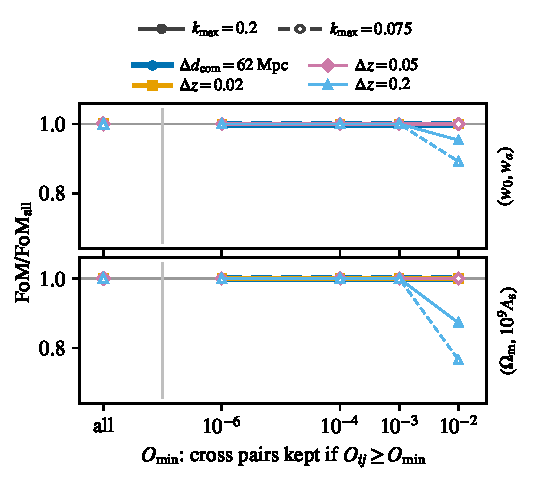
\includegraphics[width=3.5in]{plots/summary_pair_threshold/summary_pair_threshold.pdf}
  \caption{The figures of merit with only the cross pairs whose
    overlap at the fiducial dispersions reaches $O_{\min}$, over the
    current data vector's, against $O_{\min}$; ``current'', the
    current data vector, sits left of the separator.  Upper panel:
    ${\rm FoM}(w_0, w_a)$; lower: ${\rm FoM}(\Omega_m, 10^9 A_s)$; the
    panels share the $y$ axis.  Color, line width and marker: the
    layout; solid, filled markers: $\kmax = 0.2\hMpc$; dashed, open:
    $0.075$; gray: one.  \kmaxclause}
  \label{fig:pairthreshold}
\end{figure}

\paragraph{Pairs beyond the list.}
The pair list and the covariance are built once, at the fiducial
dispersions, while the model's \SigVfactor-times-wider priors allow
fits in which the kernels blur further and unmeasured pairs would
pass the overlap threshold.  Two families of longer lists measure
what such pairs are worth (Figure~\ref{fig:pairaxes}); each contains
the current data vector and grows along one axis.  The gap axis adds
every pair of bins whose raw redshift ranges are at most $g$ bin
widths apart: each step in $g$ adds the next chain of pairs, the
spectra of bins two apart at $g = 1$, three apart at $g = 2$, and so
on.  The $\sigma_v$ axis reruns the overlap criterion of
Eq.~\eqref{eq:overlap} with every dispersion set to one common value
$s$; $s$ only selects the pairs, while the model and the covariance
keep the fiducial dispersions, so this axis prices exactly the lists
that a fit carrying the dispersions toward the upper edge of their
priors would require.  Those lists change late: on
$\Delta d_{\rm com} = 62$~Mpc no pair joins until
$s = \SvJoinCom$~km/s, on $\Delta z = 0.05$ none until
$\SvJoinFive$, and on $\Delta z = 0.2$ none ever; only
$\Delta z = 0.02$ grows already at $s = \SvJoinTwo$.  On the three
thinner layouts the added pairs are worth much: at its largest list,
at the better of the two cuts the figure draws,
each layout gains a factor of \PairGainCom{},
\PairGainTwo{} and \PairGainFive{} of ${\rm FoM}(w_0, w_a)$, in
layout order, and up to \PairGainOm{} of
${\rm FoM}(\Omega_m, 10^9 A_s)$, with most of the gain in the first
added chain; on $\Delta z = 0.2$ the gain never exceeds
\PairGainTwentyMax{}.  (At $\kmax = 0.075\hMpc$ the scale cut keeps
almost no band of the pairs added on $\Delta z = 0.02$, so that
layout gains at the larger cuts.)

\begin{figure}[tbp]
  \centering
  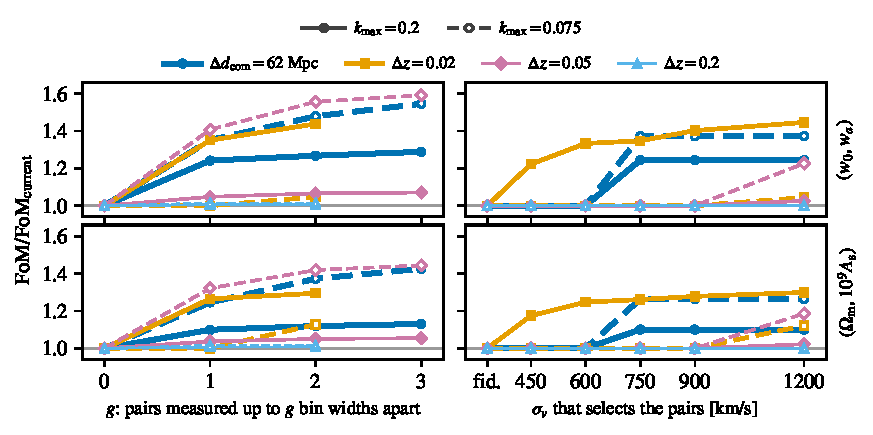
\includegraphics[width=\linewidth]{plots/summary_pair_axes/summary_pair_axes.pdf}
  \caption{The figures of merit with pairs beyond the current data
    vector, over the current data vector's, with the dispersions
    fitted.  Left column: the gap axis, pairs whose raw redshift
    ranges are at most $g$ bin widths apart; right: the $\sigma_v$
    axis, the pairs selected by the overlap criterion with every
    dispersion at the common value $s$, the model kept at the
    fiducial dispersions (``fid.'': the current selection).  Top:
    ${\rm FoM}(w_0, w_a)$; bottom: ${\rm FoM}(\Omega_m, 10^9 A_s)$;
    the panels share the $y$ axis.  Color, line width and marker: the
    layout; solid, filled markers: $\kmax = 0.2\hMpc$; dashed, open:
    $0.075$; gray: one.  \kmaxclause}
  \label{fig:pairaxes}
\end{figure}

\paragraph{Why the added pairs help.}
Besides the seven cosmological parameters, the fit determines the
nuisance parameters: the parameters that describe the galaxies
rather than the universe -- the biases, counterterms, stochastic
amplitudes and dispersions -- whose uncertainty the quoted errors
include.  The decisive ones here form each group's bias line: under
the prior of Section~\ref{sec:prior} the bias amplitudes
$\beta_i = b_{1,i} D(\bar{z}_i)$ of a group's bins follow a straight
line in redshift with a free level and a free slope -- the freedom
of the wide sample -- plus the correlated residuals the prior
charges.  The auto spectra alone cannot pin that line down.  A
higher level raises every auto spectrum of the group through
$b_{1,i}^2$ exactly as a larger clustering amplitude would, and a
slope tilts the group's spectra against each other the way an
evolving growth does -- and how growth evolves with redshift is what
$w_0$ and $w_a$ control.  The bias line and the growth history are
degenerate: they imprint nearly the same pattern on the auto
spectra, so the fit measures only a combination of them.  The
dispersions ride on the same degeneracy, since widening $\sigma_v$
lowers an auto spectrum like a lower bias does, and like a change of
$w_0$.  A cross spectrum breaks the pattern: it carries the biases
as the product $b_{1,i}\,b_{1,j}$, and its correlation coefficient
with the two auto spectra,
$C_\ell^{ij}/\sqrt{C_\ell^{ii}\,C_\ell^{jj}}$, is free of the linear
biases at linear order.  Each added pair is therefore one more
measurement of the clustering two shells share that no bias line can
reshape: it separates the bias line, and $\sigma_v$ with it, from
the growth history.  Figure~\ref{fig:pairattribution} reads the
mechanism off the forecasts.  With each group's level and slope held
at the fiducial -- the bias line fixed -- most of the gain goes: at
$\kmax = 0.075\hMpc$ the factor \PairGainFive{} of $\Delta z = 0.05$
falls to \PairLineFive{}, and the \PairGainCom{} of
$\Delta d_{\rm com} = 62$~Mpc to \PairLineCom{}; holding only the
correlated residuals fixed instead leaves the gain almost unchanged.
With every nuisance parameter fixed the added pairs keep at most
\PairNuisMax{} anywhere: the line-of-sight clustering information
the added spectra carry by themselves is worth little once the
biases are known.

\begin{figure}[tbp]
  \centering
  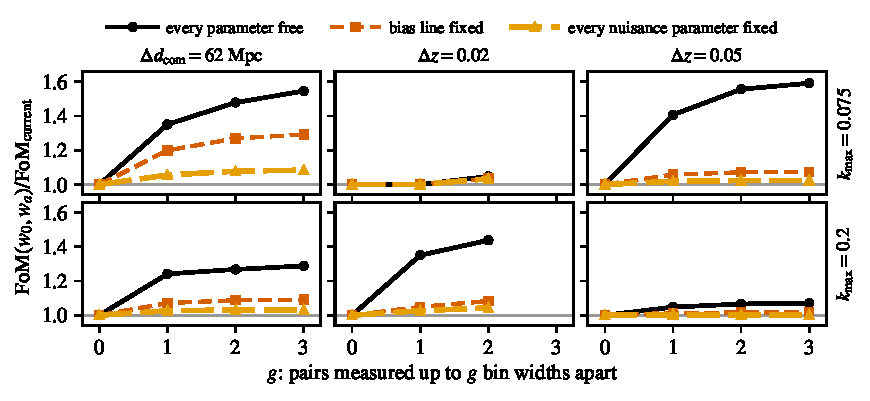
\includegraphics[width=\linewidth]{plots/summary_pair_attribution/summary_pair_attribution.pdf}
  \caption{${\rm FoM}(w_0, w_a)$ along the gap axis, over the current
    data vector's, with the dispersions fitted, on the three layouts
    whose gain is large.  Black solid, filled circles: every
    parameter free; vermillion dashed, squares: each group's bias
    line -- the level and the slope of
    $\beta_i = b_{1,i} D(\bar{z}_i)$ -- held fixed; orange
    long-dashed, triangles: every nuisance parameter held fixed.
    Rows: $\kmax = 0.075$ and $0.2\hMpc$.  \kmaxclause}
  \label{fig:pairattribution}
\end{figure}

\paragraph{What is robust, and what is open.}
The gain is a property of the bias model, not of the residual prior.
Three priors on the amplitudes pass the error-bar test of
\texttt{notes/correlated\_bias\_prior\_v2}, the test of
Section~\ref{sec:forecast} applied to each prior: this note's (the
pessimistic prior), the
baseline prior, whose residuals are smaller and correlated over a
longer length, and the free prior, with no residual prior at all.
All three leave every level and slope free, and the gain agrees
across them within about \PairPriorSpread{} of the ratio.  The
growth-tied prior -- one amplitude per group, with no slope and no
residuals -- fails that test, so no figure of merit is quoted for
it.  The analysis keeps the current data vector; the longer lists
are a comparison against it.  Open is a finite prior on the levels
and slopes, which no passing prior imposes and which would keep only
part of the gain.  The templates, tables and
checks behind these statements are in
\texttt{notes/cross\_correlations}, in its sections on what pairs
beyond the list would add and on the free bias levels and slopes.

\section{The bias model}
\label{sec:model}

\paragraph{The one-loop power spectrum.}
The galaxy power spectrum of bin $i$, in redshift space, is
\begin{align}
  P_{g,i}(k, \mu) \;={}& b_{1,i}^2\,P_{\rm mm}(k)
  + P_{\rm loop}(k;\, b_{1,i}, b_{2,i}, b_{s^2,i})
  + \alpha_{0,i}\,k^2 P_{\rm mm}(k)
  \nonumber\\
  &+ \bigl(2\,b_{1,i} f\mu^2 + f^2\mu^4\bigr) P_{\rm lin}(k)
  + \bigl(b_{1,i} + f\mu^2\bigr) f\,\alpha_{2,i}\,\mu^2 k^2
    P_{\rm lin}(k)
  \nonumber\\
  &+ \frac{1}{\bar{n}_i}\Bigl({\rm SN}_{0,i}
  + {\rm SN}_{2,i}\,f_{\rm sat}\sigma_{\rm sat}^2\,k^2\mu^2\Bigr) ,
  \label{eq:pgg}
\end{align}
with $k$ the comoving wavenumber, $\mu$ the cosine of the angle to the
line of sight, $P_{\rm mm}$ the nonlinear (halofit) matter power
spectrum, $P_{\rm lin}$ the linear one, $f = d\ln D/d\ln a$ the growth
rate and $\bar{n}_i$ the bin's number density.  $P_{\rm loop}$ holds
the one-loop terms of the quadratic bias $b_2$ and the tidal bias
$\bstwo$, the responses of the galaxy density to the squared density
contrast and to the squared tidal field~\cite{McDonaldRoy2009,Saito2014};
the third-order bias is zero.  $\alpha_0$ is the $k^2$ counterterm,
which absorbs the sensitivity of the loops to small scales.  The
$P_{\rm lin}$ terms are linear (Kaiser) redshift-space distortions on
each bin's Fingers-of-God-convolved redshift distribution, with no
redshift-space one-loop terms, and $\alpha_2$ is the line-of-sight
counterterm in the convention of the DESI 2024 full-shape
analysis~\cite{Maus2024}, in which $\alpha_2 k^2$ is a fractional
correction to the velocity part of the Kaiser power.  Equation~\eqref{eq:pgg}
writes these terms with $P_{\rm lin}$; their projection adds the Limber
difference between $P_{\rm mm}$ and $P_{\rm lin}$ (Section~\ref{sec:method}),
so where the Limber approximation holds they carry the nonlinear power.
Both counterterms are in $h^{-2}\,{\rm Mpc}^2$.  $\SNz$ is the white noise
beyond Poisson, in units of the Poisson power $1/\bar{n}_i$ that the
covariance carries, and $\SNt\,k^2\mu^2$ the stochastic term of the
satellites' velocities, in units of $f_{\rm sat}\sigma_{\rm
sat}^2/\bar{n}_i$, with $f_{\rm sat}$ the satellite fraction and
$\sigma_{\rm sat}$ the satellites' velocity dispersion in distance
units: $(\fsat, \ssatLRG\,h^{-1}{\rm Mpc})$ for LRG and
$(\fsat, \ssatELG\,h^{-1}{\rm Mpc})$ for ELG~\cite{Maus2024}, and the
LRG values for BGS.

\paragraph{The dispersions carry the line-of-sight counterterm.}
The model fixes $\alpha_2 = 0$ in every bin.  On thin bins, widening a
bin's Fingers-of-God dispersion $\sigma_v$ -- the width of the Gaussian
that smooths its redshift distribution -- damps the same line-of-sight
power that $\alpha_2$ corrects, and the two are nearly fully degenerate
in these spectra.  The model therefore samples the seven dispersions
with Gaussian priors \SigVfactor{} times their base widths (the table
of Section~\ref{sec:fiducial}; the base widths, \SigBase{}~km/s, are
five times the median per-bin uncertainty of the dispersion
measurements).  With that widening, a fit without $\alpha_2$ absorbs a
line-of-sight correction of the DESI 2024 prior size through the
dispersions alone, on every layout and at every cut; the degeneracy,
the choice of the factor and the linear-response shifts behind it are
in \texttt{notes/fog\_parameter\_degeneracy\_study}.

\paragraph{One form for every bias quantity.}
Every bias quantity $X$ of Eq.~\eqref{eq:pgg}, in bin $i$ of group
$g$, is
\begin{equation}
  X_i \;=\; X_g(\bar{z}_i) \;+\; t_{X,g}\,(\bar{z}_i - \bar{z}_g)
  \;+\; \varepsilon_{X,i} ,
  \label{eq:generic}
\end{equation}
with $X_g(\bar{z}_i)$ the group value of $X$, which includes the
calibration trend where $X$ has one, $t_{X,g}$ a tilt in redshift
across the group, $\bar{z}_g$ the mean redshift of the group's bins,
and $\varepsilon_{X,i}$ a residual of the bin.  The group value and the
tilt are the freedom of the wide sample; the residual is what thin
slicing may add within it (Section~\ref{sec:prior}).
Table~\ref{tab:params} lists what each quantity carries.

For the linear bias the three parts enter as fractions of the group
value $B_g/D(\bar{z}_i)$, which keeps the clustering amplitude $b_1 D$
constant across the group:
\begin{equation}
  b_{1,i} \;=\; \frac{B_g}{D(\bar{z}_i)}\,\bigl(1 + \delta_i\bigr),
  \qquad
  \delta_i \;=\; s_g\,(\bar{z}_i - \bar{z}_g) + \varepsilon_i ,
  \label{eq:linear}
\end{equation}
with $B_g$ the group amplitude, $s_g$ the tilt, $\varepsilon_i$ the
residual and $\delta_i$ the fractional deviation from the group value.
The group values of the quadratic and tidal biases are calibrations
evaluated at the bin's own linear bias, plus a group offset:
\begin{equation}
  b_{2,i} = b_2^{\rm L}(b_{1,i}) + \Delta_{2,g}
    + t_{2,g}\,(\bar{z}_i - \bar{z}_g) ,
  \qquad
  b_{s^2,i} = -\tfrac{4}{7}\,\bigl(b_{1,i} - 1\bigr) + \Delta_{s,g}
    + t_{s,g}\,(\bar{z}_i - \bar{z}_g) ,
  \label{eq:calibrations}
\end{equation}
with $b_2^{\rm L}(b_1) = 0.412 - 2.143\,b_1 + 0.929\,b_1^2 +
0.008\,b_1^3$ the separate-universe fit of Lazeyras et
al.~\cite{Lazeyras2016} and the second relation the co-evolution of a
population formed with local bias~\cite{Saito2014}.  Only the linear
bias carries a residual of its own: the quadratic and tidal biases
receive each bin's residual through $b_{1,i}$ in their calibrations,
and the counterterms and stochastic terms have none.

\begin{table}[tbp]
  \centering
  \begin{tabular}{llll}
    \toprule
    quantity & group value & tilt & residual \\
    \midrule
    $b_1$ & $B_g/D(\bar{z}_i)$; $B_g$ flat & $s_g$, flat
      & $\varepsilon_i$, Eq.~\eqref{eq:kernel} \\
    $b_2$ & $b_2^{\rm L}(b_{1,i}) + \Delta_{2,g}$; $\Delta_{2,g}$ width
      \wDtwo{} & flat & none of its own \\
    $\bstwo$ & $-\tfrac{4}{7}(b_{1,i} - 1) + \Delta_{s,g}$;
      $\Delta_{s,g}$ width \wDs{} & flat & none of its own \\
    $\alpha_0$ & width $\ctFrac/\kmax^2$ & flat & none \\
    $\alpha_2$ & fixed to $0$ & none & none \\
    $\SNz$ & width \wSNz{} & none & none \\
    $\SNt$ & width \wSNt{} & none & none \\
    \bottomrule
  \end{tabular}
  \caption{What each bias quantity carries in Eq.~\eqref{eq:generic}.
    A width is that of a Gaussian prior centered on zero, so the
    fiducial model sits on the calibrations with no counterterm and no
    stochastic term beyond Poisson; flat marks a flat prior.  The
    $\alpha_0$ width is the rule of the DESI 2024 full-shape
    analysis~\cite{DESI2024V,Maus2024}, a correction of $\ctFrac$ at
    the cut, evaluated at each cut ($\ctDESI\aunit$ at $0.2\hMpc$).
    $\alpha_2$ is fixed: the widened dispersion priors carry its
    freedom.  A
    group of one bin has no tilt.}
  \label{tab:params}
\end{table}

\paragraph{Why $\SNt$ matters on thin bins.}
A constant power $N$ projects exactly as
$N \int d\chi\, W_i W_j/\chi^2$ onto bins $i$ and $j$, with $\chi$ the
comoving distance and $W_i(\chi)$ the Fingers-of-God-convolved kernel
of bin $i$; bins of two different
samples share no stochastic term.  A power proportional to
$k^2\mu^2 = k_\parallel^2$ is that of the line-of-sight derivative of a
white noise, so $\SNt$ projects with each kernel replaced by its
derivative, $W_i' = dW_i/d\chi$:
\begin{equation}
  C_\ell^{ij}\big|_{\SNt} \;=\; U_{ij} \int d\chi\,
  \frac{W_i'(\chi)\,W_j'(\chi)}{\chi^2} ,
  \label{eq:sn2}
\end{equation}
with $U_{ij}$ the mean of the two bins' amplitudes
$\SNt f_{\rm sat}\sigma_{\rm sat}^2/\bar{n}$.  A thin bin's $W_i'$
peaks at its two edges with opposite signs, and adjacent bins share an
edge, where one kernel rises as the other falls: the projected $\SNt$
of neighbors is anticorrelated.  Normalized by the two auto terms, the
adjacent term has a median of $\SNtAdj$ over the \NadjPairs{} adjacent
pairs of one sample on $\Delta d_{\rm com} = 62$~Mpc, against $\SNzAdj$
for $\SNz$.  No white noise, per group or per bin, mimics this pattern,
and a fit without $\SNt$ is biased on the thin layouts already at
$\kmax = 0.075\hMpc$ (\texttt{notes/higher\_order\_bias}).

\section{The prior: the freedom of the wide sample}
\label{sec:prior}

\paragraph{The principle.}
DESI selects each group as one wide sample, and what is known about
its bias, from calibrations to the priors of full-shape analyses,
refers to that sample.  Slicing it into thin bins adds measurements of
the clustering, not knowledge of the bias.  A thin-bin prior is
therefore fair only if it leaves each group the freedom of its wide
sample, whatever the slicing.  In Eq.~\eqref{eq:generic} that freedom
is the group value and the tilt, whose priors are set for the wide
sample; the residual is what the slicing may add within it, local
features of the size the selection can produce, and its prior must not
tighten as the bins get thinner.

\paragraph{The linear bias.}
The level $B_g$ and the tilt $s_g$ are free, and the residual has a
Gaussian prior, zero across groups and correlated within one,
\begin{equation}
  \bigl\langle \varepsilon_i\,\varepsilon_j \bigr\rangle
  \;=\; \sigma_g^2\,
  \exp\!\left(-\,\frac{|\bar{z}_i - \bar{z}_j|}{L}\right) ,
  \label{eq:kernel}
\end{equation}
with $\sigma_g$ the width of one bin's residual and $L$ the correlation
length in redshift.  The kernel defines a random process
$\varepsilon(z)$ along each group before any binning, which a layout
only samples at its bin redshifts: the prior on a coarse set of
redshifts is the marginal of the prior on a finer one, so slicing finer
adds no prior knowledge.  Two neighbors at separation $\Delta z$ differ
by an rms $\sigma_g[2(1 - e^{-\Delta z/L})]^{1/2}$.  The prior charges
only the residual around each group's best straight line
(Section~\ref{sec:method}), so a group of one or two bins, as on
$\Delta z = 0.2$, has a free bias in every bin.

No measurement resolves the bias of these samples below
$\Delta z \approx \MeasuredDz$, so the sizes come from what selects
them (\texttt{notes/correlated\_bias\_prior\_v2}).  Coherent changes
move a whole group along a nearly straight line, which the free tilt
absorbs: a conserved population, whose bias obeys
$b_1 - 1 \propto 1/D$~\cite{Fry1996}, departs from $B_g/D$ by about
\ConsDrift{} per $\Delta z = 0.05$, and the $r < 19.5$ flux limit of
BGS~\cite{Hahn2023} drifts its bias by \BGSspan{} across the group.
Local changes, such as the 4000~\AA\ break crossing a filter edge over
$\Delta z \approx \FilterDzMin$--$\FilterDzMax$, move bins
independently.  Hence $\sigma_g = \sigG$ in every group, above the
largest derived departure from a line (the \BGScurv{} rms that the BGS
flux limit leaves), and $L = \Lcorr$, the scale of a filter-edge
crossing; neighbors at $\Delta z = 0.02$ then differ by \NeighborRms{}
rms.  The draws of Figure~\ref{fig:draws} keep the line of the known
drift and add local features of a few percent.

\begin{figure}[tbp]
  \begin{minipage}[c]{3.3in}
    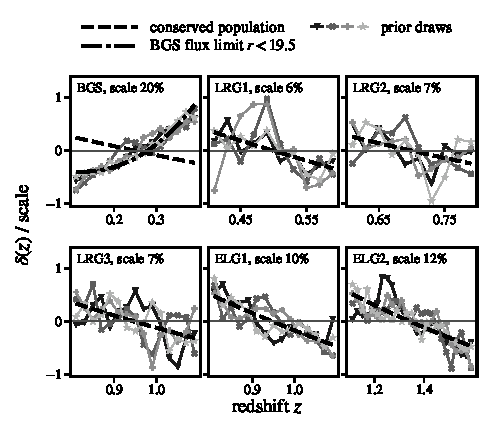
\includegraphics{plots/summary_prior_draws/summary_prior_draws.pdf}
  \end{minipage}\hfill
  \begin{minipage}[c]{\dimexpr\linewidth-3.3in-\sidegap\relax}
  \captionsetup{justification=raggedright,singlelinecheck=false}
  \caption{Four draws of the prior on the $\Delta z = 0.02$ bins, one
    panel per group, each panel divided by the round scale written in
    it.  Thick black dashed: the conserved-population drift; thick
    black dash-dot (BGS only): the $r < 19.5$ flux-limit drift.  Thin
    gray lines: the draws of $\delta(z)$, each with its own shade, line
    width and marker.  Every
    draw keeps the best straight line through its group's reference
    drift, the flux limit in BGS and the conserved population
    elsewhere, and differs from it by a residual drawn with
    $\sigma_g = \sigG$ and $L = \Lcorr$.  The level of every curve is
    removed, since $B_g$ is free.}
  \label{fig:draws}
  \end{minipage}
\end{figure}

\paragraph{The higher-order terms.}
The calibrations of $b_2$ and $\bstwo$ describe halo populations; a
wide sample adds how far it sits from them.  Each group therefore gets
one offset per family, with the widths of Table~\ref{tab:params}:
twice what the known imperfection of the calibrations requires (the
scatter of the Lazeyras fit and the \CoevSpread{} spread between
co-evolution and excursion-set tidal biases), so that the calibrations
act as prior centers where the loops reach \LoopShare{} of the galaxy
power.  A calibration of the wide sample says nothing about how the
offset changes inside it, so the tilt is free; it also absorbs exactly
a calibration that drifts linearly across a group.  The counterterm
$\alpha_0$ follows the same pattern, since its scale follows the host
halos of the selection.  The stochastic amplitudes do not tilt: their
Poisson part is known bin by bin.

\section{Projection, covariance and the Fisher forecast}
\label{sec:method}

\paragraph{Non-Limber spectra.}
The Limber approximation evaluates the power spectrum only at the
transverse wavenumber $(\ell + 1/2)/\chi$ and misses the
line-of-sight modes that a thin bin with sharp edges passes.  The
exact projection keeps them: between bins $i$ and
$j$, with $W_i(\chi) = n_i(z)\,dz/d\chi$ the radial kernel of bin $i$,
$n_i$ its normalized redshift distribution, $j_\ell$ the spherical
Bessel function and $P(k;\, z_1, z_2)$ the unequal-time power spectrum
of the projected field at $z_1 = z(\chi_1)$ and $z_2 = z(\chi_2)$,
\begin{equation}
  C_\ell^{ij} \;=\; \frac{2}{\pi} \int d\chi_1\, W_i(\chi_1)
  \int d\chi_2\, W_j(\chi_2)
  \int_0^\infty dk\, k^2\, P(k;\, z_1, z_2)\,
  j_\ell(k\chi_1)\, j_\ell(k\chi_2) .
  \label{eq:exactcl}
\end{equation}
The double Bessel integral is the cost: $j_\ell(k\chi_1)\,
j_\ell(k\chi_2)$ oscillates and beats, and quadrature over it is slow
and unstable.

Fang et al.~\cite{FangKEM2020} (FKEM) remove that cost by splitting
the spectrum into its linear part and a nonlinear remainder.  The
linear part is separable, $P_{\rm lin}(k;\, z_1, z_2) =
D(z_1)\,D(z_2)\,P_{\rm lin}(k)$, with $P_{\rm lin}(k)$ the linear
matter power spectrum today, so in Eq.~\eqref{eq:exactcl} each
$\chi$ integral closes around its own Bessel function and becomes a
one-dimensional transform that the FFTLog algorithm computes quickly.
The remainder $P_{\rm mm} - P_{\rm lin}$, with $P_{\rm mm}$ the
nonlinear matter power spectrum, matters only at high $k$, which
projects to multipoles where the Limber approximation is accurate, so
it is added in Limber:
\begin{equation}
  C_\ell \;=\; C_\ell^{\rm exact}[P_{\rm lin}]
  \;+\; C_\ell^{\rm Limber}[P_{\rm mm}]
  \;-\; C_\ell^{\rm Limber}[P_{\rm lin}] .
  \label{eq:fkem}
\end{equation}

FKEM projects three transfer kernels per galaxy bin: density,
redshift space and magnification.  The density and redshift-space
(Kaiser) parts together give, with $b_{1,i}$ the bin's linear galaxy
bias and $f = d\ln D/d\ln a$ the linear growth rate ($a$ the scale
factor),
\begin{equation}
  \Delta_\ell^i(k) \;=\; \int d\chi\, W_i(\chi)\, D(z)
  \left[\, b_{1,i}\, j_\ell(k\chi) \;-\; f(z)\, j_\ell''(k\chi)
  \,\right] :
  \label{eq:kaiserkernel}
\end{equation}
each factor $f\mu^2$ of the flat-sky Kaiser power, with $\mu$ the
cosine of the angle to the line of sight, becomes a $-j_\ell''$ in the
exact projection.  In the Limber terms of Eq.~\eqref{eq:fkem} the
identity $j_\ell''(x) = [\ell(\ell-1)/x^2 - 1]\,j_\ell(x)
+ (2/x)\,j_{\ell+1}(x)$ writes the second derivative with the orders
$\ell$ and $\ell+1$, and Limber evaluates each order at its own
distance, $\chi_\ell = (\ell + 1/2)/k$ and
$\chi_{\ell+1} = (\ell + 3/2)/k$, so the Limber redshift-space kernel
combines the bin's radial kernel at two neighbouring distances:
redshift-space distortions move galaxies between neighbouring shells.
The third kernel, lensing magnification, is proportional to
the magnification bias $b_{\rm mag}$, the response of the observed
number density to the lensing convergence; this forecast sets
$b_{\rm mag} = 0$ in every DESI bin and every LSST Y1 lens bin, so
magnification is neglected.

For thin bins the split of Eq.~\eqref{eq:fkem} is not enough.
Limber's error shrinks with the width of the radial kernel, so for a
thin bin the Limber remainder stays wrong far past the switch
multipole: the hand-off fails exactly where accuracy was the goal.
The density--density part of every DESI spectrum -- the linear-bias
term, the one-loop terms and the $\alpha_0$ counterterm of
Eq.~\eqref{eq:pgg} -- is therefore projected by a low-rank
factorization instead.  Per bin, a singular value decomposition writes
the square root of the real-space galaxy power spectrum $P_g(k, z)$ as
a sum of five products of a function of $k$ and a function of $z$,
each projected with its own FFTLog transform; the unequal-time
spectrum is the geometric mean
$\sqrt{P_g(k, z_1)}\,\sqrt{P_g(k, z_2)}$, exact at equal times and
treating the two fields as fully correlated otherwise.  This carries
the full one-loop power with no Limber hand-off up to a multipole cap
at $\ell = 1000$, below which every kept band lies.

The hybrid in one sentence: the density--density part runs through the
low-rank factorization; the Kaiser terms and the $\alpha_2$
counterterm keep the FKEM split, projected exactly with
$P_{\rm lin}$ and corrected in Limber by Eq.~\eqref{eq:fkem}; the
stochastic terms are projected as exact templates; and magnification
is neglected.  The one-loop power is not pushed through the velocity
terms because velocities do not grow like the density field once
nonlinear.

\paragraph{The covariance.}
The band-power covariance is Gaussian, computed at the one-loop
fiducial (every bin's linear bias on its group's trend, $b_2$ and
$\bstwo$ on their calibrations, every other bias term zero) for
\AreaCov{} square degrees, with its inverse rescaled to the forecast's
\AreaSurvey{}.  The data vectors are the model's own prediction at
that fiducial.

\paragraph{The Fisher matrix.}
Let $\mathbf{m}(\mathbf{p})$ be the model band powers at the parameters
$\mathbf{p}$, $\mathbf{p}_0$ the fiducial point, $\mathsf{C}$ the
band-power covariance, and $\mathsf{D} = \partial\mathbf{m}/\partial
\mathbf{p}$ at $\mathbf{p}_0$ (sans-serif, unlike the growth factor
$D$).  At a scale cut that keeps the set $K$ of band powers, the Fisher
matrix of a fit is
\begin{equation}
  F \;=\; \mathsf{D}_K\T\,\mathsf{C}_{KK}^{-1}\,\mathsf{D}_K
  \;+\; F_{\rm prior} ,
  \label{eq:fisher}
\end{equation}
with $\mathsf{D}_K$ the kept rows of $\mathsf{D}$ and $\mathsf{C}_{KK}$
the kept block of $\mathsf{C}$.  $F_{\rm prior}$ adds
$1/\sigma_{\rm pr}^2$ to the diagonal for a Gaussian prior of width
$\sigma_{\rm pr}$ and nothing for a flat one.  For each group and each
quantity that carries a residual (Table~\ref{tab:params}) it adds the
precision $\mathsf{P} = \mathsf{Q} - \mathsf{Q}\mathsf{U}(\mathsf{U}\T
\mathsf{Q}\mathsf{U})^{-1}\mathsf{U}\T\mathsf{Q}$ on the bins'
deviations from the group value ($\delta_i$ for $b_1$), with
$\mathsf{Q}$ the inverse kernel matrix of Eq.~\eqref{eq:kernel} and
$\mathsf{U}$ the matrix with columns $1$ and $\bar{z}_i - \bar{z}_g$:
it charges only the residual around the group's best straight line.
The marginalized error of parameter $j$ is
$\sigma_j = [(F^{-1})_{jj}]^{1/2}$, and the FoMs of
Section~\ref{sec:data} are $[\det \mathsf{C}_p]^{-1/2}$, with
$\mathsf{C}_p$ the $2 \times 2$ block of $F^{-1}$ of the two
parameters.  Where a cut leaves a combination of nuisance parameters
without information, for instance the flat tilts of a group most of
whose bins have lost their bands, $F$ is inverted as a pseudo-inverse:
scaled to unit diagonal, diagonalized, and restricted to the
eigen-directions above $\PinvTol$ of the largest eigenvalue.  A dropped
direction may not touch $(w_0, w_a)$, $\Omega_m$ or $A_s$ by more than
$\PinvTouch$; otherwise the cut gives no fit.

\paragraph{Derivatives.}
The columns of $\mathsf{D}$ come from three kinds of derivatives at the
fiducial point.
\begin{enumerate}
  \item The cosmological parameters, the $\sigma_v$ and the per-bin
    $b_{1,i}$, $b_{2,i}$, $b_{s^2,i}$ and $\alpha_{0,i}$, on which the
    band powers depend nonlinearly, take the five-point central stencil
    \begin{equation}
      \frac{\partial\mathbf{m}}{\partial\theta} \;\simeq\;
      \frac{\mathbf{m}(\theta_0 - 2\epsilon)
        - 8\,\mathbf{m}(\theta_0 - \epsilon)
        + 8\,\mathbf{m}(\theta_0 + \epsilon)
        - \mathbf{m}(\theta_0 + 2\epsilon)}{12\,\epsilon} ,
      \label{eq:stencil}
    \end{equation}
    with $\theta_0$ the fiducial value and $\epsilon = h\,\theta_0$,
    $h = \StepH$ (an absolute step where $\theta_0 = 0$); its truncation
    error is of order $\epsilon^4$.  Every evaluation is a full call of
    the likelihood, CAMB included.
  \item $\SNz$, $\SNt$ and $\alpha_2$ enter linearly, so their columns
    are exact: the projected templates per unit amplitude for the
    stochastic terms (Eq.~\eqref{eq:sn2} for $\SNt$), and a two-point
    difference for $\alpha_2$.
  \item The per-bin columns are computed in batches.  A spectrum
    $C^{ij}_\ell$ depends on the biases of bins $i$ and $j$ only, so the
    bins of a set $\mathcal{S}$ in which no two bins share a measured
    spectrum can be stepped together.  With $\partial_{\mathcal{S}}
    \mathbf{m}$ the stencil of Eq.~\eqref{eq:stencil} with the bias $x$
    stepped in every bin of $\mathcal{S}$,
    \begin{equation}
      \frac{\partial m_r}{\partial x_i} \;=\;
      \begin{cases}
        (\partial_{\mathcal{S}}\mathbf{m})_r & \text{if band power $r$
          belongs to a spectrum that contains bin } i \in \mathcal{S} ,
          \\
        0 & \text{otherwise.}
      \end{cases}
      \label{eq:batch}
    \end{equation}
    A greedy coloring of the graph of measured pairs gives \Nbatch{}
    such batches on every layout, so each per-bin family costs
    \NevalFamily{} evaluations, whatever the number of bins.
\end{enumerate}

\paragraph{One base, every model.}
The columns of one layout, for the cosmology, the $\sigma_v$ and the
seven per-bin families $b_1$, $b_2$, $\bstwo$, $\alpha_0$, $\alpha_2$,
$\SNz$ and $\SNt$, form a base matrix $\mathsf{B}$, computed once and
cached.  A model is a fixed linear map from its parameters $p_j$ to the
base quantities $\kappa_a$,
\begin{equation}
  \mathsf{D} \;=\; \mathsf{B}\,\mathsf{M} ,
  \qquad
  \mathsf{M}_{aj} \;=\; \frac{\partial\kappa_a}{\partial p_j} :
  \label{eq:dbm}
\end{equation}
a group offset puts ones on its group's bins in its family's block, a
tilt the weights $\bar{z}_i - \bar{z}_g$, a bin's linear bias the chain
rule through the calibrations of Eq.~\eqref{eq:calibrations}, and the
untied versions of Section~\ref{sec:grouping} per-bin identities.  With
$\mathsf{G}_K = \mathsf{B}_K\T\mathsf{C}_{KK}^{-1}\mathsf{B}_K$ computed
once per cut, every model and prior at that cut has
$F = \mathsf{M}\T\mathsf{G}_K\mathsf{M} + F_{\rm prior}$: a change of
model, prior, cut or truth needs no new evaluation of the data vector.

\paragraph{Shifts and the error-bar test.}
A truth that departs from the fitted model moves the band powers by
$\Delta\mathbf{m}$, and the best fit, to first order, by
\begin{equation}
  \delta\mathbf{p} \;=\; F^{-1}\,\mathsf{D}_K\T\,\mathsf{C}_{KK}^{-1}\,
  \Delta\mathbf{m}_K ,
  \label{eq:shift}
\end{equation}
exactly for the terms linear in their amplitude ($\alpha_2$, $\SNz$,
$\SNt$) and to first order for the biases, on which the band powers
depend quadratically.  Because $\delta\mathbf{p}$ is linear in the
truth, the average behind the error-bar test of
Section~\ref{sec:forecast} is exact in closed form; for
$(w_0, w_a)$,
\begin{equation}
  \langle\chi^2\rangle \;=\; \Delta_{\rm drift}^2
  \;+\; {\rm tr}\bigl[\mathsf{C}_p^{-1}\bigl(\mathsf{A}\,\Sigma\,
  \mathsf{A}\T + \mathsf{N}_p\bigr)\bigr] ,
  \label{eq:chi2}
\end{equation}
with $\Delta_{\rm drift}$ the shift of the known drift alone in units
of the ellipse, $\mathsf{A}$ the response of $(w_0, w_a)$ to the bins'
deviations $\delta_i$, $\Sigma$ the covariance of the residuals drawn
from the prior, and $\mathsf{N}_p$ the $(w_0, w_a)$ block of
$F^{-1}F_0F^{-1}$, the share of the data noise and the other priors,
$F_0$ being $F$ without the correlated prior.  For $\Omega_m$ or $A_s$
the same holds with the parameter's own row.

\paragraph{Numerical convergence.}
Noise in the data vector, from its integration grids and CAMB's
tolerances, enters a finite difference divided by the step.  A column
$\mathbf{d}_j + \mathbf{e}_j$ with noise $\mathbf{e}_j$ raises $F_{jj}$
on average by $\langle\mathbf{e}_j\T\mathsf{C}^{-1}\mathbf{e}_j\rangle
> 0$: noise reads as information and inflates the FoM.  Settings that
converge a $\chi^2$ to the standard of MCMC runs,
$|\Delta\chi^2| < \MCMCdchi$, are therefore not enough.  On
$\Delta z = 0.05$ they inflate ${\rm FoM}(w_0, w_a)$ by \ConvMCMCLow{}
at $\kmax = 0.075\hMpc$ and \ConvMCMCHigh{} at $0.2\hMpc$; the excess
comes from
noise in the $w_0$, $w_a$ and $\Omega_m$ columns.  That spurious
information also weakens the degeneracies the error bars rest on, such
as the one between the dispersions and the cosmology, which is why the
final settings are
needed.  The criterion of
convergence is step independence: the FoMs, the errors and the shifts
must not move when the stencil step changes or the numerical controls
are refined further.  A study on $\Delta z = 0.05$
(Figure~\ref{fig:convergence}) starts from a configuration with every
control raised: the grid factor $g = \GridStart$, where $g$ counts the
comoving distances of the non-Limber integrals in units of
\GridUnit{}; CosmoLike's \texttt{accuracyboost} \StartAccBoost{} and
\texttt{integration\_accuracy} \StartIntAcc{}; the low-rank engine's
rank \StartRank{} and multipole cap \StartCap{}; and CAMB's
\texttt{AccuracyBoost} \StartCambBoost{}, \texttt{k\_per\_logint}
\StartKlog{} and maximum wavenumber \StartKmax{}~Mpc$^{-1}$.  From
there it changes one control at a time and compares each configuration
with the converged value, the five-point stencil at step $h$ on
$g = \GridConv$.  The final settings are:
\begin{itemize}
  \setlength{\itemsep}{1pt}
  \item the final grid $g = \GridFinal$, \GridRatio{} times the MCMC grid of
    $\Delta z = 0.05$, with CosmoLike's \texttt{accuracyboost}
    \FinAccBoost{} and \texttt{integration\_accuracy} \FinIntAcc{};
  \item CAMB's \texttt{AccuracyBoost} \FinCambBoost{},
    \texttt{k\_per\_logint} \FinKlog{} and a maximum wavenumber of
    \FinKmax{}~Mpc$^{-1}$, with halofit's bisection tolerance tightened
    from $\HalofitStock$ to $\HalofitPatch$ (the halofit tolerance
    patch);
  \item five-point stencils for every stencil and per-bin column.
\end{itemize}
Against the converged value they give ${\rm FoM}(w_0, w_a)$
\ConvFoMwLow{} at $\kmax = 0.075\hMpc$ and \ConvFoMwHigh{} at
$0.2\hMpc$ (${\rm FoM}(\Omega_m, 10^9 A_s)$ \ConvFoMoLow{} and
\ConvFoMoHigh{}), marginalized errors within \ConvSigma{} and shifts
within $\ConvShift\sigma$.  From step $h/2$ to $3h$ both FoMs stay
within \ConvStep{} on $\Delta z = 0.05$, and from $h/2$ to $2h$ within
\ConvStepCom{} on
$\Delta d_{\rm com} = 62$~Mpc.  Two cross-checks agree.  DerivKit,
which fits a polynomial through at least \DkitPoints{} evaluations
around the fiducial point, matches the stencils within \DkitAgree{}.
The study's route, which unties the per-bin parameters in the
likelihood, matches the production route, which steps them through
CosmoLike's setter: exactly for $b_2$, $\bstwo$ and $\alpha_0$, within
$\RouteBone$ for $b_1$ and within $\RouteStencil$ for the stencil
columns.

\begin{figure}[tbp]
  \begin{minipage}[c]{3.78in}
    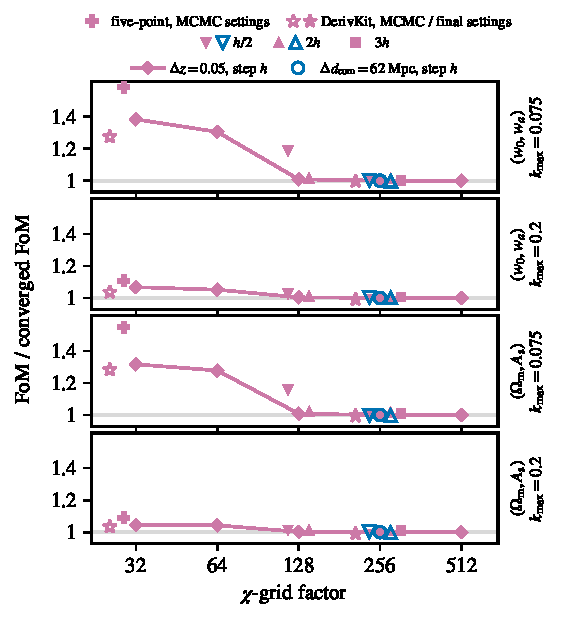
\includegraphics{plots/fom_convergence/fom_convergence.pdf}
  \end{minipage}\hfill
  \begin{minipage}[c]{\dimexpr\linewidth-3.78in-\sidegap\relax}
  \captionsetup{justification=raggedright,singlelinecheck=false}
  \caption{Convergence of the forecast on $\Delta z = 0.05$: the FoMs
    of the model divided by their converged values (five-point stencils
    at step $h$ on the grid factor $g = \GridConv$).  From the top,
    ${\rm FoM}(w_0, w_a)$ and ${\rm FoM}(\Omega_m, 10^9 A_s)$ at
    $\kmax = 0.075$ and $0.2\hMpc$.  Diamonds on the line: the scan in
    $g$ at step $h$, which holds every other control at the study's
    starting configuration ($g = \GridStart$ with the other controls
    raised; Section~\ref{sec:method}); $g = \GridFinal$ is the final
    setting.  Filled down-triangles,
    up-triangles and squares beside a grid: steps $h/2$, $2h$ and $3h$.
    Plus: five-point stencils at the MCMC settings.  Open and filled
    stars: DerivKit at the MCMC and at the final settings.  Open blue
    markers: $\Delta d_{\rm com} = 62$~Mpc at the final settings, steps
    $h/2$ (down-triangle) and $2h$ (up-triangle) against its own step-$h$
    value (ring).  Gray band: $1 \pm 1\%$.  \kmaxclause}
  \label{fig:convergence}
  \end{minipage}
\end{figure}

\paragraph{Cost.}
A layout's base takes \Neval{} evaluations of the data vector, about
\TevalMin{} to \TevalMax{}~s each at the final settings, so \HoursMin{}
to \HoursMax{} hours per thin layout; every model, prior, cut and truth
then costs a fraction of a second.  \texttt{notes/fisher\_machinery}
gives the details.

\section{Forecast}
\label{sec:forecast}

\paragraph{Figures of merit.}
Figure~\ref{fig:fom} draws both FoMs against $\kmax$.
${\rm FoM}(w_0, w_a)$ is \FoMwLowCom{}, \FoMwLowTwo{}, \FoMwLowFive{}
and \FoMwLowTwenty{} at $\kmax = 0.075\hMpc$ and \FoMwHighCom{},
\FoMwHighTwo{}, \FoMwHighFive{} and \FoMwHighTwenty{} at $0.2\hMpc$, in
layout order ($\Delta d_{\rm com} = 62$~Mpc, $\Delta z = 0.02$, $0.05$,
$0.2$); ${\rm FoM}(\Omega_m, 10^9 A_s)$ at $0.2\hMpc$ is
\FoMoHighCom{}, \FoMoHighTwo{}, \FoMoHighFive{} and \FoMoHighTwenty{}.
The thin layouts carry most of the information.  LSST Y1 3x2pt alone
gives \LSSTw{} and \LSSTo{}; DESI $C_\ell^{gg}$ alone stays below it in both
FoMs at every cut.

\begin{figure}[tbp]
  \begin{minipage}[c]{3.46in}
    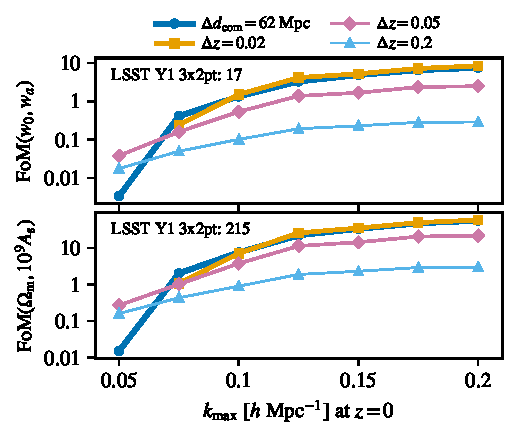
\includegraphics{plots/summary_fom_kmax/summary_fom_kmax.pdf}
  \end{minipage}\hfill
  \begin{minipage}[c]{\dimexpr\linewidth-3.46in-\sidegap\relax}
  \captionsetup{justification=raggedright,singlelinecheck=false}
  \caption{${\rm FoM}(w_0, w_a)$ (top) and
    ${\rm FoM}(\Omega_m, 10^9 A_s)$ (bottom) of DESI $C_\ell^{gg}$ alone
    against $\kmax$.  Color, line width and marker: the layouts.  Text in
    each panel: LSST Y1 3x2pt alone.  On
    $\Delta z = 0.02$ the cut at $0.05$ keeps no band.  \kmaxclause}
  \label{fig:fom}
  \end{minipage}
\end{figure}

\paragraph{The error bars are honest.}
How well a fit's quoted error bars cover where the fit actually lands
is measured by $\eta = \chidof$, with
$\chi^2 = \Delta p\T \mathsf{C}_p^{-1} \Delta p$, $\Delta p$ the
recovered minus the true parameters, $\mathsf{C}_p$ the fit's
marginalized covariance, $n_{\rm dof} = 2$ for $(w_0, w_a)$ and $1$
for $\Omega_m$ or $A_s$, and $\langle\cdot\rangle$ the average over the
truths and the data noise; $\eta = 1$ for honest error bars.  Over
random bias histories, the known drifts plus a residual drawn from the
prior, $\eta \le \EtaMax$ at every cut and on every layout (at most
\EtaW{} for $(w_0, w_a)$, \EtaOm{} for $\Omega_m$ and \EtaAs{} for
$A_s$), and the $1\sigma$ region covers the truth in at least
\CoverMin{} of universes, against $68.3\%$ for honest error bars.

\section{What the grouping is worth}
\label{sec:grouping}

The principle of Section~\ref{sec:prior} says that a thin-bin prior
must keep the freedom of the wide original samples, and add nothing to
it.  Figure~\ref{fig:untied} puts the principle to a test on six
versions of the priors: five untie the bias bin by bin, and one ties it
harder, to a constant across each sample.  The top two rows divide each
version's FoM by the model's; the bottom row asks whether its error
bars are honest, with the statistic $\eta$ of
Section~\ref{sec:forecast} for $(w_0, w_a)$ over the same random bias
histories.  The group width of a parameter is the width the model gives
it (Table~\ref{tab:params}), and $N$ is the number of bins of its
group.  The first four versions free $b_{1,i}$ in every bin and give
$\Delta_2$, $\Delta_s$, $\alpha_0$, $\SNz$ and $\SNt$ one
value per bin; the fifth keeps the model whole, its $b_1$ prior
included; the sixth ties every bin of a sample to one value.  Every
version keeps the model's dispersion priors, with no $\alpha_2$.

\begin{figure}[tbp]
  \centering
  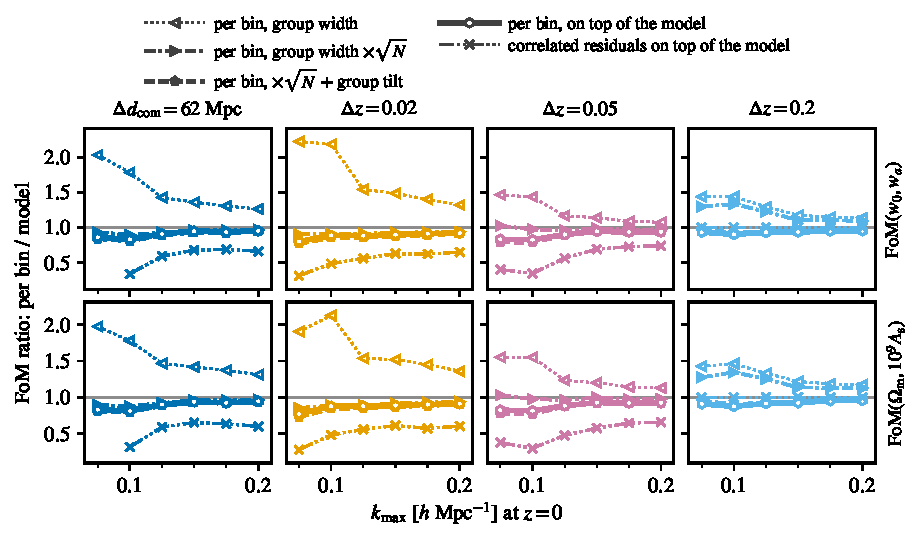
\includegraphics{plots/summary_fom_untied/summary_fom_untied.pdf}
  \caption{Six versions of the bias priors against the model, one
    column per layout.  Top and middle rows: ${\rm FoM}(w_0, w_a)$ and
    ${\rm FoM}(\Omega_m, 10^9 A_s)$, each divided by the model's.
    Bottom row: $\eta = \chidof$ of $(w_0, w_a)$ over the random bias
    histories of Section~\ref{sec:forecast}; for the constant version
    the truth also holds the bias's own evolution inside each sample.
    The group width is the width the model gives a group parameter, and
    $N$ the number of bins of the group.  The first four versions free
    $b_{1,i}$ in each bin and give $\Delta_2$, $\Delta_s$, $\alpha_0$,
    $\SNz$ and $\SNt$ one value per bin.  Dotted, open left
    triangles: the group width; dash-dot, filled right triangles: the
    group width times $\sqrt{N}$; dashed, filled pentagons: the same
    plus a free tilt per group; solid, open hexagons: the group width
    on top of the model's offsets and tilts.  The line width grows in
    that order.  Thin dash-dot-dot line, crosses: the model, its $b_1$
    prior included, plus correlated per-bin residuals on $\Delta_2$,
    $\Delta_s$ and $\alpha_0$.  Thick long-dashed line, plus
    signs: one constant value of every bias quantity per wide sample.
    Thin gray line: a ratio of $1$, and honest error bars in the bottom
    row.  There the other five versions coincide at $1$; the solid
    line, drawn on top, hides all but the crosses.  The cuts start at
    $\kmax = 0.075\hMpc$: at $0.05\hMpc$ the model's own
    ${\rm FoM}(w_0, w_a)$ is below \FoMwSmallCut{}.  \kmaxclause}
  \label{fig:untied}
\end{figure}

\paragraph{Why a naive per-bin prior gains.}
Give each of $N$ bins its own offset, independent of the others, each
with a Gaussian prior of width $\sigma$.  Their average is the sum of
the $N$ offsets divided by $N$.  Variances of independent numbers add,
so the sum has variance $N\sigma^2$ and the average
$N\sigma^2/N^2 = \sigma^2/N$: the average has width $\sigma/\sqrt{N}$.
With $\sigma = \wDtwo$, the group width of $\Delta_2$, and
$N = \ToyN$, the prior pins the group's average offset to $\ToyAvg$,
\ToyFactor{} times tighter than the wide sample knows it.  Slice the same sample into more bins and the
pin tightens further, with no new knowledge of the bias.

\paragraph{The six versions,} in the words of the figure's legend:
\begin{itemize}
  \item \textbf{per bin, group width}: looks looser than the model, but
    pins each group's average to the group width over $\sqrt{N}$.  It
    lies above the model on every layout and at every cut, by up to a
    factor of \UntieGainMax{}: a gain by accident, from the slicing.
  \item \textbf{per bin, group width $\times\sqrt{N}$}: gives each
    group's average back the group width.  On $\Delta z = 0.2$, whose
    groups hold one or two bins, it still gains, because it fixes the
    trend inside a group that the model leaves free.
  \item \textbf{per bin, $\times\sqrt{N}$ + group tilt}: frees that
    trend too, and so restores the whole wide-sample freedom.  Its
    prior is at least as loose as the model's in every direction (each
    bin's variance is $N$ times the squared group width, against one
    squared group width for the shift common to all bins), so it can
    only lose FoM.
  \item \textbf{per bin, on top of the model}: keeps the model's group
    offsets and tilts, the wide-sample freedom, and adds an independent
    per-bin value of the group width to every term.
  \item \textbf{correlated residuals on top of the model}: keeps the
    model exactly and adds to each of $\Delta_2$, $\Delta_s$ and
    $\alpha_0$ a per-bin residual with the prior of
    $b_1$'s: Gaussian, of the term's group width, correlated in redshift
    over $L = \LcorrHO$, and charged only on the deviations from the
    group's line.  In the form of Eq.~\eqref{eq:generic} it fills the
    residual column of Table~\ref{tab:params} for these three terms.  In
    a group of one or two bins the offset and the tilt already fix
    every bin, so on $\Delta z = 0.2$ this version is the model.
  \item \textbf{one constant value per wide sample}: every thin bin of
    a group shares one value of every bias quantity, constant in
    redshift.  The linear bias is a plain constant, $b_{1,i} = B_g$
    instead of $B_g/D(\bar{z}_i)$, and $\Delta_2$, $\Delta_s$,
    $\alpha_0$, $\SNz$ and $\SNt$ take one value per group,
    under the model's priors on the group values, with no tilts and no
    residuals.  It is the simplest way to slice a wide sample.
\end{itemize}

\paragraph{What untying the bins costs.}
The last two versions keep the wide-sample freedom and add only the
freedom of untied bins, so they measure what untying really costs, and
they differ sharply.  Independent per-bin terms on top of the model
cost a factor of \CostNestedLowMin{} to \CostNestedLowMax{} in
${\rm FoM}(w_0, w_a)$ on the thin layouts at $\kmax = 0.075\hMpc$, and
\CostNestedHighMin{} to \CostNestedHighMax{} on the three thinner
layouts at $0.2\hMpc$.  Correlated residuals cost a factor of
\CostCorrLowMin{} to \CostCorrLowMax{} on the three thinner layouts at
$0.075\hMpc$, the most on $\Delta z = 0.02$, and
\CostCorrHighMin{} to \CostCorrHighMax{} on the same layouts at
$0.2\hMpc$.
A residual that is smooth in redshift can mimic a change of the
cosmology across neighboring bins, while independent per-bin terms
average down over the bins of a group.  On $\Delta z = 0.2$ neither
version costs more than a factor of \CostWideMax{} at any cut.

\paragraph{What a constant per sample claims.}
The sixth version claims the largest gains of the figure:
\ConstGainLowMin{} to \ConstGainLowMax{} times the model's
${\rm FoM}(w_0, w_a)$ over the layouts at $\kmax = 0.075\hMpc$,
\ConstGainHighMin{} to \ConstGainHighMax{} at $0.2\hMpc$, and
\ConstGainOmMin{} to \ConstGainOmMax{} times
${\rm FoM}(\Omega_m, 10^9 A_s)$.  The bottom row prices the claim.  For
this version the truth also holds the evolution of the bias inside each
sample, which a constant cannot follow: the fiducial bias itself
evolves, the linear bias as $B_g/D(\bar{z}_i)$, and $b_2$ and $\bstwo$
with it through the calibrations.  That evolution alone shifts
$(w_0, w_a)$ by \ConstEvoLowMin{} to \ConstEvoLowMax{}$\sigma$ at
$0.075\hMpc$ and \ConstEvoHighMin{} to \ConstEvoHighMax{}$\sigma$ at
$0.2\hMpc$; the known drifts partly cancel it, which is why $\eta$
comes out smaller than those shifts.  The error bars are still
\ConstEtaLowMin{} to \ConstEtaLowMax{} times too small at $0.075\hMpc$
and \ConstEtaHighMin{} to \ConstEtaHighMax{} at $0.2\hMpc$, where they
reach \ConstEtaOm{} for $\Omega_m$ and \ConstEtaAs{} for $A_s$, and the
$68.3\%$ region covers the truth in \ConstCoverMin{} to \ConstCoverMax{}
of universes (\ConstCoverWorst{} at the worst, on
$\Delta z = 0.02$).  The
gain is the information the evolution of the bias would have to supply,
asserted instead by the prior: where the model keeps the freedom the
bias has on the wide original samples, a constant removes even the
freedom the wide sample's own evolution needs.  Even $\Delta z = 0.2$,
one or two bins per sample, gains a factor of \ConstGainTwentyMin{} to
\ConstGainTwentyMax{} and fails the test: giving up the tilts and the
residuals there gives up real freedom.

\paragraph{What the bottom row tests.}
The random truths change only the linear bias, so the bottom row tests
the linear bias, not the higher-order terms.  The four versions that
free $b_{1,i}$ per bin sit exactly at $1$ by construction: a free
per-bin linear bias absorbs any change of the linear bias, so their
honesty there says nothing about their higher-order freedom.  The
version with correlated residuals, whose $b_1$ keeps the model's prior,
stays between \EtaCorrMin{} and \EtaCorrMax{}, and the model itself at
most \EtaW{} (Section~\ref{sec:forecast}).

\section{Where the details are}
\label{sec:details}

\begin{itemize}
  \setlength{\itemsep}{1pt}
  \item \texttt{notes/correlated\_bias\_prior\_v2}: the linear-bias
    prior and its physics, the projected precision, the random bias
    histories and the error-bar test, and the comparisons of priors and
    models.
  \item \texttt{notes/higher\_order\_bias}: the one-loop model, its
    calibrations, the size and exact projection of every term, and its
    validation.
  \item \texttt{notes/linear\_bias\_kmax}: the reach of linear bias,
    which motivates the one-loop terms.
  \item \texttt{notes/fisher\_machinery}: the Fisher derivatives, their
    convergence study, and the assembly of every Fisher matrix, shift
    and $\langle\chi^2\rangle$.
  \item \texttt{notes/cross\_correlations}: which thin-bin pairs the data
    vector measures, the Fingers-of-God blur, and the study of pairs
    beyond the list -- the gap and $\sigma_v$ axes, the attribution of
    the gain to the free bias levels and slopes, and the comparison
    across the linear-bias priors.
  \item \texttt{notes/fog\_parameter\_degeneracy\_study}: the degeneracy
    of the line-of-sight counterterm $\alpha_2$ with the dispersions
    $\sigma_v$, the choice of their prior widths, and the
    linear-response shifts that estimate how safe a chain run with this
    model would be.
\end{itemize}

\footnotesize
\raggedright
\begin{thebibliography}{99}
\setlength{\itemsep}{1pt}

\bibitem{Asorey2012}
J.~Asorey, M.~Crocce, E.~Gazta\~naga and A.~Lewis,
``Recovering 3D clustering information with angular correlations'',
2012, arXiv:1207.6487.

\bibitem{FangKEM2020}
X.~Fang, E.~Krause, T.~Eifler and N.~MacCrann,
``Beyond Limber: efficient computation of angular power spectra for
galaxy clustering and weak lensing'',
2020, arXiv:1911.11947.

\bibitem{DESCSRD2018}
The LSST Dark Energy Science Collaboration,
``The LSST Dark Energy Science Collaboration (DESC) Science
Requirements Document'',
2018, arXiv:1809.01669.

\bibitem{Saraivanov2026}
E.~Saraivanov, H.~Rubira, V.~Miranda and T.~Eifler,
``Towards the Two-Loop EFTofLSS in Galaxy Lensing Surveys'',
2026, arXiv:2603.13031.

\bibitem{DeRoseChen2025}
J.~DeRose and S.~Chen,
``The Lensing Counter Narrative: An Effective Description of
Small-Scale Clustering in Weak Lensing Power Spectra'',
2025, arXiv:2510.18981.

\bibitem{McDonaldRoy2009}
P.~McDonald and A.~Roy,
``Clustering of dark matter tracers: generalizing bias for the coming
era of precision LSS'',
2009, arXiv:0902.0991.

\bibitem{Saito2014}
S.~Saito, T.~Baldauf, Z.~Vlah, U.~Seljak, T.~Okumura and P.~McDonald,
``Understanding higher-order nonlocal halo bias at large scales by
combining the power spectrum with the bispectrum'',
2014, arXiv:1405.1447.

\bibitem{Maus2024}
M.~Maus, S.~Chen, M.~White et al.,
``An analysis of parameter compression and full-modeling techniques
with Velocileptors for DESI 2024 and beyond'',
2024, arXiv:2404.07312.

\bibitem{Lazeyras2016}
T.~Lazeyras, C.~Wagner, T.~Baldauf and F.~Schmidt,
``Precision measurement of the local bias of dark matter halos'',
2016, arXiv:1511.01096.

\bibitem{DESI2024V}
DESI Collaboration,
``DESI 2024 V: Full-shape galaxy clustering from galaxies and
quasars'',
2024, arXiv:2411.12021.

\bibitem{Fry1996}
J.~N.~Fry,
``The Evolution of Bias'',
1996, ApJ, 461, L65.

\bibitem{Hahn2023}
C.~Hahn et al.,
``The DESI Bright Galaxy Survey: Final Target Selection, Design, and
Validation'',
2023, AJ, 165, 253,
arXiv:2208.08512.

\end{thebibliography}

\end{document}
